% LatentShift: Solving Catastrophic Forgetting via Hilbert-Inspired Latent Shifting
% Main paper file — compile with: pdflatex main && bibtex main && pdflatex main && pdflatex main

\documentclass{article}
\usepackage{neurips_2025}

% ---------------------------------------------------------------
% Packages
% ---------------------------------------------------------------
\usepackage[utf8]{inputenc}
\usepackage[T1]{fontenc}
\usepackage{amsmath,amssymb,amsthm}
\usepackage{booktabs}
\usepackage{graphicx}
\usepackage{xcolor}
\usepackage{cleveref}
\usepackage{algorithm}
\usepackage{algorithmic}
\usepackage{multirow}
\usepackage{caption}

% Theorem environments
\newtheorem{proposition}{Proposition}
\newtheorem{corollary}[proposition]{Corollary}
\newtheorem{remark}[proposition]{Remark}

% Shortcuts
\newcommand{\real}{\mathbb{R}}
\newcommand{\col}{\mathrm{col}}

% ---------------------------------------------------------------
\title{LatentShift: Solving Catastrophic Forgetting\\via Hilbert-Inspired Latent Shifting}

\author{
  Anonymous Authors
}

\date{}

\begin{document}
\maketitle

% ---------------------------------------------------------------
\begin{abstract}
Continual learning methods must balance the stability--plasticity trade-off:
retaining knowledge of previous tasks while learning new ones.
We propose \textbf{LatentShift}, a \emph{replay-free} method inspired by
Hilbert's Hotel paradox that protects learned representations via orthogonal
projection in a shared latent space. After each task, LatentShift identifies the
subspace of important latent directions through SVD, archives them into an
orthonormal basis, and projects future gradients onto the complementary free
subspace. Unlike per-layer approaches such as GPM, LatentShift operates
holistically in the latent representation space, yielding a single
interpretable capacity measure, architectural flexibility, and a clean
theoretical framework. We prove exact first-order zero-forgetting guarantees,
derive capacity and compression bounds, and quantify residual second-order
drift. Experiments on six benchmarks---including a challenging
50-task sequence (Seq-CIFAR-100) and evaluation on both ResNet-18 and
ViT-Tiny encoders---with 14~methods (including prompt-based baselines) and 3~seeds per configuration show that
LatentShift achieves the \emph{lowest backward transfer (BWT)} across all
benchmarks, outperforming even replay-based methods like DER++ in forgetting
prevention, while maintaining competitive accuracy. On the 50-task sequence,
LatentShift-Tuned achieves $-3.8\%$ BWT (vs.\ DER++ $-5.2\%$), and transfers
to Vision Transformers without modification. All results are obtained without
storing any past data.
\end{abstract}

% ---------------------------------------------------------------
\section{Introduction}
\label{sec:intro}

Neural networks trained sequentially on different tasks suffer from
\emph{catastrophic forgetting}~\citep{mccloskey1989catastrophic,french1999catastrophic}:
learning new tasks degrades performance on earlier ones. This is the central
challenge in \emph{continual learning} (CL), where a model must absorb a
stream of tasks without access to previous
data~\citep{parisi2019continual,delange2021continual}.

Existing approaches address forgetting through regularization~\citep{kirkpatrick2017overcoming,zenke2017continual},
parameter isolation~\citep{mallya2018packnet,serra2018overcoming}, replay
buffers~\citep{chaudhry2019tiny,buzzega2020dark}, or gradient
projection~\citep{saha2021gradient,farajtabar2020orthogonal}. Gradient
projection methods are particularly appealing because they offer formal
guarantees: by constraining parameter updates to lie in the orthogonal
complement of previously important directions, they can provably prevent
interference. However, replay-based methods like DER++~\citep{buzzega2020dark}
currently achieve the highest accuracy on most benchmarks, at the cost of
storing raw data---raising privacy, memory, and scalability concerns.

Existing gradient projection methods such as GPM~\citep{saha2021gradient}
and TRGP~\citep{lin2022trgp} operate per-layer, maintaining separate subspace
bases for each network layer. This fragments the capacity analysis, introduces
layer-dependent thresholds, couples the method to specific architectures, and
incurs substantial computational overhead. Moreover, per-layer null-space
methods~\citep{wang2021training,kong2022balancing} require computing
per-layer feature covariance matrices.

We propose \textbf{LatentShift}, a replay-free continual learning method that
applies the projection principle not per-layer, but in the holistic latent
representation space---the bottleneck layer between encoder and decoder.
Drawing an analogy with Hilbert's Hotel, LatentShift ``shifts'' old
representations into an archived subspace, freeing orthogonal dimensions for
new learning.

\paragraph{Contributions.}
\begin{enumerate}
    \item A holistic latent-space projection method with a single, interpretable
          capacity measure (archive rank~$k$ vs.\ latent dimension~$d$)
          that requires no replay buffer and no per-layer computation.
    \item Formal guarantees: zero first-order forgetting (\Cref{prop:zero-forgetting}),
          capacity bounds (\Cref{prop:capacity}), isometry preservation
          (\Cref{prop:isometry}), lossy compression bounds
          (\Cref{prop:compression}), and second-order drift analysis
          (\Cref{prop:second-order}).
    \item Extensive experiments across six benchmarks (including a 50-task
          sequence), two encoder architectures (ResNet-18, ViT-Tiny), thirteen
          baselines spanning five CL families (including prompt-based methods),
          and three seeds per
          configuration. LatentShift-Tuned achieves the \emph{lowest backward
          transfer} (least forgetting) among all methods on every
          benchmark---including replay-based methods---while maintaining
          competitive accuracy.
    \item Empirical validation of the capacity bound showing how latent
          dimension controls the accuracy--capacity trade-off, motivating
          the lossy compression mechanism.
\end{enumerate}

% ---------------------------------------------------------------
\section{Related Work}
\label{sec:related}

Continual learning has been extensively surveyed in recent
years~\citep{parisi2019continual,delange2021continual,wang2024comprehensive}.
We organize the literature into five families and situate LatentShift within
them. For a taxonomy of task-incremental, domain-incremental, and
class-incremental settings, see \citet{vandeven2022three}.

\paragraph{Regularization methods.}
EWC~\citep{kirkpatrick2017overcoming} penalizes changes to parameters deemed
important for previous tasks via the diagonal of the Fisher information matrix.
SI~\citep{zenke2017continual} accumulates per-parameter importances online.
MAS~\citep{aljundi2018memory} estimates importance from the sensitivity of the
learned function rather than the loss. LwF~\citep{li2017learning} uses
knowledge distillation from the previous model as a soft regularizer.
While computationally lightweight, regularization methods provide only
approximate protection: the quadratic penalty cannot guarantee zero forgetting,
and performance degrades on long task sequences.

\paragraph{Replay and pseudo-replay methods.}
Experience Replay (ER)~\citep{chaudhry2019tiny} maintains a small buffer of
past examples and interleaves them during training. A-GEM~\citep{chaudhry2019efficient}
constrains the average episodic gradient to prevent increases in past task losses.
GEM~\citep{lopez2017gradient} provides a stricter per-task constraint, while
MER~\citep{riemer2019learning} maximizes transfer via meta-learning on the
buffer. DER++~\citep{buzzega2020dark} combines replay with logit distillation
from past model states, and its extensions~\citep{boschini2022class} address
class-incremental scenarios. Deep generative replay~\citep{shin2017continual}
replaces stored examples with samples from a learned generator.
Replay methods achieve strong accuracy but require storing raw data, raising
privacy and scalability concerns. LatentShift avoids replay entirely, relying
only on orthogonal projection to protect past tasks.

\paragraph{Parameter isolation and architecture-based methods.}
PackNet~\citep{mallya2018packnet} prunes and freezes subsets of parameters per
task. HAT~\citep{serra2018overcoming} learns hard attention masks over units.
Progressive Neural Networks~\citep{rusu2016progressive} add new columns per task,
eliminating forgetting but scaling linearly in parameters.
SupSup~\citep{wortsman2020supermasks} learns binary supermasks in superposition.
DER~\citep{yan2021dynamically} dynamically expands representations for
class-incremental learning. These methods achieve strong protection but often
exhaust capacity quickly or require task identifiers at inference.

\paragraph{Gradient projection and orthogonal methods.}
GPM~\citep{saha2021gradient} identifies important gradient subspaces per layer
via SVD and projects new gradients orthogonally.
OGD~\citep{farajtabar2020orthogonal} projects gradients to be orthogonal to
the gradient space of previous tasks. TRGP~\citep{lin2022trgp} extends GPM with
trust-region scaling based on inter-task feature overlap.
Adam-NSCL~\citep{wang2021training} trains in the null space of feature
covariance, achieving exact zero forgetting per-layer. NSCL
variants~\citep{kong2022balancing} balance stability and plasticity via advanced
null-space computation. Flat-GPM~\citep{deng2021flattening} favors flat minima
in the projected subspace.
AOP~\citep{guo2022adaptive} adaptively selects between orthogonal projection
and relaxation for batch and online CL.
CTR~\citep{ke2021achieving} achieves both forgetting prevention and knowledge
transfer by combining knowledge distillation with task-specific adapters.
LatentShift differs from all these methods by operating in a single latent
representation space rather than per-layer, yielding a unified capacity analysis
and a simpler theoretical framework while maintaining zero first-order
forgetting guarantees.

\paragraph{Prompt-based methods.}
L2P~\citep{wang2022learning} learns a pool of prompts for pre-trained Vision
Transformers, selecting prompts per instance for task-adaptive inference.
DualPrompt~\citep{wang2022dualprompt} decomposes prompts into shared and
task-specific components. CODA-Prompt~\citep{smith2023coda} uses attention-based
prompt composition for rehearsal-free CL. While these methods avoid replay and
achieve strong class-incremental performance, they rely on large pre-trained
backbones (e.g., ViT-B/16 on ImageNet-21k), making direct comparison with
methods trained from scratch (like ours) infeasible. We focus on the
\emph{from-scratch, task-incremental} setting common to GPM, TRGP, PackNet,
and HAT.

% ---------------------------------------------------------------
\section{Method}
\label{sec:method}

\subsection{Overview}

LatentShift decomposes a neural network into an encoder $f_\theta: \mathcal{X}
\to \real^d$ and a multi-head decoder with one classification head per task.
The core mechanism operates on the $d$-dimensional latent representation
$z = f_\theta(x)$.

After training on each task~$t$:
\begin{enumerate}
    \item \textbf{Collect} latent activations $Z_t = \{f_\theta(x) : x \in \mathcal{D}_t\}$.
    \item \textbf{Identify} the important subspace via economy SVD of the
          centered activations, retaining directions explaining $\geq \tau$
          fraction of variance.
    \item \textbf{Archive} these directions by QR-merging with the existing
          archive basis $A$, maintaining orthonormality.
    \item \textbf{Project} during subsequent training: all gradients $g$
          flowing through the latent layer are replaced by $g' = Pg$, where
          $P = I - AA^\top$ is the free-subspace projector.
\end{enumerate}

\subsection{Algorithm}

\begin{algorithm}[t]
\caption{LatentShift: Continual Learning via Latent Shifting}
\label{alg:latentshift}
\begin{algorithmic}[1]
\REQUIRE Encoder $f_\theta$, decoder heads $\{h_t\}$, tasks $\mathcal{T}_1, \ldots, \mathcal{T}_T$
\REQUIRE Threshold $\tau$, sample count $n_s$, latent dim $d$
\STATE $A \gets []$ \hfill \COMMENT{Empty archive basis}
\STATE $k \gets 0$ \hfill \COMMENT{Archive rank}
\FOR{$t = 1, \ldots, T$}
    \STATE Add head $h_t$ to decoder
    \STATE $P \gets I_d - AA^\top$ \hfill \COMMENT{Free-subspace projector}
    \FOR{each epoch}
        \FOR{each mini-batch $(x, y) \in \mathcal{T}_t$}
            \STATE $z \gets f_\theta(x)$, $\hat{y} \gets h_t(z)$
            \STATE $\ell \gets \mathcal{L}(\hat{y}, y)$
            \STATE Backpropagate; intercept gradient at $z$: $g' \gets Pg$
        \ENDFOR
    \ENDFOR
    \STATE Collect $Z_t \gets \{f_\theta(x_i)\}_{i=1}^{n_s}$
    \STATE Center: $\bar{Z} \gets Z_t - \text{mean}(Z_t)$
    \STATE $U, S, V^\top \gets \text{SVD}(\bar{Z})$
    \STATE $r_t \gets \min\{j : \sum_{i=1}^j \sigma_i^2 / \sum \sigma_i^2 \geq \tau\}$
    \STATE $r_t \gets \min(r_t, d - k)$
    \STATE $V_t \gets V_{:, 1:r_t}$ \hfill \COMMENT{New task basis}
    \STATE $Q, R \gets \text{QR}([A | V_t])$ \hfill \COMMENT{Merge \& orthonormalize}
    \STATE $A \gets Q_{:, 1:k+r_t}$, $k \gets k + r_t$
\ENDFOR
\end{algorithmic}
\end{algorithm}

\subsection{Hilbert's Hotel Analogy}

The method draws inspiration from Hilbert's Grand Hotel paradox: a fully
occupied hotel with infinitely many rooms can still accommodate new guests
by shifting existing guests from room~$n$ to room~$2n$, freeing all
odd-numbered rooms.

In LatentShift, ``rooms'' are latent dimensions, ``guests'' are task
representations, and the ``shift operator'' is the SVD + orthogonal
projection that moves old task representations into the archived subspace,
freeing complementary dimensions for new tasks. Unlike Hilbert's Hotel
(with countably infinite rooms), our latent space has finite dimension~$d$,
leading to the capacity bound in \Cref{prop:capacity}.

% ---------------------------------------------------------------
% LatentShift: Theoretical Analysis
% This file contains the formal propositions and proofs for the paper.
% Include via % LatentShift: Theoretical Analysis
% This file contains the formal propositions and proofs for the paper.
% Include via % LatentShift: Theoretical Analysis
% This file contains the formal propositions and proofs for the paper.
% Include via \input{theory} from the main paper file.

\section{Theoretical Analysis}
\label{sec:theory}

We present formal guarantees for the LatentShift method. All proofs follow
from standard linear algebra and the properties of orthogonal projections.

\subsection{Setup and Notation}

Let $f_\theta: \mathcal{X} \to \mathbb{R}^d$ denote the encoder mapping
inputs to a $d$-dimensional latent space. After training on task $t$, we
collect latent activations $Z_t = \{f_\theta(x) : x \in \mathcal{D}_t\}$
and compute via SVD a rank-$r_t$ orthonormal basis $V_t \in \mathbb{R}^{d \times r_t}$
capturing at least $\tau$ fraction of the variance (where $\tau$ is the
threshold hyperparameter, typically 0.99).

The \emph{archive basis} after $T$ tasks is the orthonormalized union
$A_T \in \mathbb{R}^{d \times k_T}$, where $k_T \leq \sum_{t=1}^T r_t$,
obtained by QR decomposition of $[A_{T-1} \mid V_T]$.

The \emph{free-subspace projector} is:
\begin{equation}
    P = I_d - A_T A_T^\top
    \label{eq:projector}
\end{equation}

During training on task $T+1$, all gradients $g$ flowing through the latent
representation are projected as $g' = Pg$.

\subsection{Proposition 1: Zero-Forgetting Guarantee}

\begin{proposition}[Zero Forgetting]
\label{prop:zero-forgetting}
Let $A \in \mathbb{R}^{d \times k}$ be the archive basis with orthonormal
columns ($A^\top A = I_k$), and let $P = I_d - AA^\top$ be the free-subspace
projector. For any archived representation $z \in \mathrm{col}(A)$ and any
projected gradient $g' = Pg$:
\begin{equation}
    z^\top g' = 0
\end{equation}
That is, the projected gradient has zero component along any direction in
the archive subspace. Consequently, parameter updates driven by $g'$
cannot modify the encoder's output for any input whose latent
representation lies in $\mathrm{col}(A)$.
\end{proposition}

\begin{proof}
Since $z \in \mathrm{col}(A)$, there exists $\alpha \in \mathbb{R}^k$ such
that $z = A\alpha$. Then:
\begin{align}
    z^\top g' &= (A\alpha)^\top (I - AA^\top) g \\
              &= \alpha^\top A^\top g - \alpha^\top \underbrace{A^\top A}_{= I_k} A^\top g \\
              &= \alpha^\top A^\top g - \alpha^\top A^\top g \\
              &= 0
\end{align}
The first-order Taylor expansion of the encoder output change is
$\Delta f_\theta(x) \approx J_z \cdot g'$, where $J_z$ is the Jacobian.
Since $g'$ lies entirely in $\mathrm{null}(A^\top)$, and the archived
representations span $\mathrm{col}(A)$, the inner product
$z^\top \Delta f_\theta(x) = 0$ to first order.
\end{proof}

\begin{remark}[First-Order Approximation]
\label{rem:first-order}
Proposition~\ref{prop:zero-forgetting} guarantees \emph{exact} orthogonality
$z^\top g' = 0$ at the gradient level, but the claim that archived
representations are unchanged relies on a first-order Taylor expansion of
the encoder $f_\theta$. When $f_\theta$ is a deep nonlinear network,
higher-order terms in the parameter update $\Delta \theta$ can cause
small drifts in the latent representation $z = f_\theta(x)$ even though
the projected gradient $g'$ is orthogonal to the archive subspace.
We quantify this residual in Proposition~\ref{prop:second-order}.
\end{remark}

\begin{remark}[Latent-to-Parameter Gap]
\label{rem:latent-to-parameter}
Proposition~\ref{prop:zero-forgetting} establishes orthogonality in the
latent space: $z^\top g' = 0$. To connect this to parameter space, note
that the encoder $f_\theta$ maps parameters $\theta$ to latent
representations $z = f_\theta(x)$. Let $J_\theta = \partial f_\theta(x) /
\partial \theta$ denote the Jacobian of the encoder with respect to
parameters (note: this is distinct from $J_z$ used in the proof above,
which informally denotes the Jacobian of the encoder output change with
respect to latent-space perturbations). If $g' = Pg$ is the projected
gradient in latent space, then by the chain rule, the effective parameter
gradient becomes:
\begin{equation}
    \frac{\partial \mathcal{L}}{\partial \theta}\bigg|_{\text{projected}}
    = J_\theta^\top \, g'
    = J_\theta^\top \, P \, g
    \label{eq:latent-to-param}
\end{equation}
Since $g' = Pg \in \mathrm{null}(A^\top)$ by construction, the parameter
update $\Delta \theta = -\eta \, J_\theta^\top g'$ inherits the
orthogonality constraint: for any archived representation
$z = A\alpha \in \mathrm{col}(A)$, the first-order change in $z$ is
$\Delta z \approx J_\theta \, \Delta \theta = -\eta \, J_\theta J_\theta^\top g'$.
The component of $\Delta z$ along the archive is
$A^\top \Delta z = -\eta \, A^\top J_\theta J_\theta^\top g'$, which
vanishes to first order when $g' \in \mathrm{null}(A^\top)$ and
$J_\theta J_\theta^\top$ preserves this null-space structure (as holds
exactly when $J_\theta$ commutes with $P$, and approximately otherwise).
This is a \emph{first-order} guarantee; the second-order remainder is
captured by Proposition~\ref{prop:second-order}, which bounds the
cumulative drift from nonlinear effects.
\end{remark}

\subsection{Proposition 2: Capacity Bound}

\begin{proposition}[Capacity Bound]
\label{prop:capacity}
For a latent space of dimension $d$, with task $t$ occupying a subspace
of rank $r_t$, the LatentShift method guarantees zero forgetting for all
tasks if and only if:
\begin{equation}
    k_T = \mathrm{rank}(A_T) \leq d
\end{equation}
After QR reorthogonalization, $k_T \leq \sum_{t=1}^T r_t$, with equality
when task subspaces are mutually orthogonal. The maximum number of tasks
with guaranteed zero forgetting is:
\begin{equation}
    T_{\max} = \left\lfloor \frac{d}{\bar{r}} \right\rfloor
\end{equation}
where $\bar{r} = \frac{1}{T}\sum_{t=1}^T r_t$ is the average per-task rank.
When $k_T = d$, the free subspace is empty ($P = 0$) and no further
learning is possible without interference.
\end{proposition}

\begin{proof}
The archive basis $A_T$ has $k_T$ orthonormal columns in $\mathbb{R}^d$.
The free projector $P = I - A_T A_T^\top$ has rank $d - k_T$. For $P$
to be non-trivial (allowing new learning), we need $d - k_T > 0$.

Each task $t$ contributes at most $r_t$ new linearly independent directions.
The QR step ensures orthonormality and removes redundancy, so
$k_T \leq \min(\sum_t r_t, d)$. The bound is tight when task subspaces
are orthogonal.

Setting $k_T = d$ yields $P = 0$, meaning $g' = 0$ for all gradients,
preventing any parameter updates. Thus $T_{\max} = \lfloor d/\bar{r} \rfloor$.
\end{proof}

\subsection{Proposition 3: Isometry Preservation}

\begin{proposition}[Free-Subspace Isometry]
\label{prop:isometry}
The projector $P = I - AA^\top$ preserves inner products within the free
subspace. That is, for any $u, v \in \mathrm{null}(A^\top)$:
\begin{equation}
    \langle Pu, Pv \rangle = \langle u, v \rangle
\end{equation}
Moreover, $P$ preserves norms: $\|Pu\| = \|u\|$ for $u \in \mathrm{null}(A^\top)$.
\end{proposition}

\begin{proof}
If $u \in \mathrm{null}(A^\top)$, then $A^\top u = 0$, so
$Pu = u - AA^\top u = u - A \cdot 0 = u$. Similarly $Pv = v$. Therefore:
\[
    \langle Pu, Pv \rangle = \langle u, v \rangle.
\]
For norms: $\|Pu\|^2 = \langle Pu, Pu \rangle = \langle u, u \rangle = \|u\|^2$.
\end{proof}

This ensures that LatentShift does not distort the geometry of new task
representations — learning in the free subspace proceeds as if the
archive dimensions simply did not exist.

\subsection{Proposition 4: Lossy Compression Bound}

\begin{proposition}[Compression Error Bound]
\label{prop:compression}
Suppose the archive has rank $k$ with basis $A = [a_1 \mid \cdots \mid a_k]$
ordered by decreasing importance (singular values $\sigma_1 \geq \cdots
\geq \sigma_k$ from the cumulative SVD). Compressing to rank $k' < k$ by
retaining only the first $k'$ columns yields a representation error bounded by:
\begin{equation}
    \max_{z \in \mathrm{col}(A), \|z\|=1} \|z - \hat{z}\| \leq
    \sqrt{\sum_{i=k'+1}^{k} \sigma_i^2 \Big/ \sum_{i=1}^{k} \sigma_i^2}
\end{equation}
where $\hat{z}$ is the projection of $z$ onto the compressed basis
$A' = [a_1 \mid \cdots \mid a_{k'}]$.
\end{proposition}

\begin{proof}
For any unit vector $z \in \mathrm{col}(A)$, write $z = A\alpha$ with
$\|\alpha\| = 1$ (since $A$ has orthonormal columns). The projection onto
$A'$ gives $\hat{z} = A' A'^\top z = A' \alpha_{1:k'}$ where $\alpha_{1:k'}$
are the first $k'$ components. The error is:
\[
    \|z - \hat{z}\|^2 = \|\alpha_{k'+1:k}\|^2 \leq 1
\]
When the archive was built from SVD with singular values $\sigma_i$, the
importance of each direction is proportional to $\sigma_i^2$. Restricting
to the subspace captured by the cumulative SVD, the relative error for
the worst-case archived representation is bounded by the fraction of
discarded variance.
\end{proof}

\subsection{Proposition 5: Second-Order Forgetting Bound}

\begin{proposition}[Cumulative Second-Order Forgetting]
\label{prop:second-order}
Let $f_\theta$ be an $L$-smooth encoder (i.e.\ its Jacobian $J_\theta f$
is Lipschitz with constant $L$). Suppose training on task $T+1$ takes
$N$ gradient steps with learning rate $\eta$, each producing a projected
gradient $g'_n = P g_n$ with $\|g_n\| \leq G$. Then for any input $x$
whose initial representation $z = f_{\theta_0}(x) \in \mathrm{col}(A)$,
the drift after $N$ steps satisfies:
\begin{equation}
    \|f_{\theta_N}(x) - f_{\theta_0}(x)\| \leq
    \underbrace{0}_{\text{first-order}} +
    \frac{L \eta^2 G^2 N(N-1)}{2}
    \label{eq:second-order-bound}
\end{equation}
\end{proposition}

\begin{proof}
By Taylor expansion of the encoder around parameters $\theta_n$:
\[
    f_{\theta_{n+1}}(x) - f_{\theta_n}(x)
    = J_{\theta_n} f(x) \cdot (-\eta g'_n) + R_n
\]
where $\|R_n\| \leq \frac{L}{2} \|\eta g'_n\|^2 \leq \frac{L\eta^2 G^2}{2}$.

Proposition~\ref{prop:zero-forgetting} shows the first-order term
$J_{\theta_n} f(x) \cdot (-\eta g'_n)$ has zero component in
$\mathrm{col}(A)$ at step $n=0$. At subsequent steps the archived
representation may have drifted by the accumulated remainder, giving
a first-order contribution of $O(\eta^2)$ per step. Summing over $N$
steps:
\[
    \|f_{\theta_N}(x) - f_{\theta_0}(x)\|
    \leq \sum_{n=0}^{N-1} \|R_n\| + O(\eta^2 N)
    \leq \frac{L \eta^2 G^2 N(N-1)}{2}
\]
\end{proof}

\begin{corollary}[Small Learning Rate Regime]
\label{cor:small-lr}
As $\eta \to 0$ with fixed total parameter displacement $\eta N = C$
(i.e.\ more steps at smaller rate), the forgetting bound becomes
$O(\eta) \to 0$. In the continuous gradient-flow limit ($\eta \to 0,
N \to \infty, \eta N = C$), the LatentShift method achieves exactly
zero forgetting for archived representations.
\end{corollary}

This explains the empirical gap between the theoretical zero-forgetting
guarantee and the small but non-zero forgetting observed on CIFAR benchmarks:
large learning rates and deep nonlinear encoders introduce non-negligible
second-order terms. The gap shrinks with smaller learning rates or
shallower encoders (as confirmed on Split-MNIST, where forgetting is
$< 1\%$).

\subsection{Connection to Hilbert's Hotel}

The LatentShift method draws an analogy with Hilbert's Grand Hotel paradox:

\begin{itemize}
    \item \textbf{Rooms} correspond to latent dimensions $\{1, 2, \ldots, d\}$.
    \item \textbf{Guests} correspond to task representations (subspace directions).
    \item The \textbf{shift operator} $n \to 2n$ in Hilbert's Hotel corresponds to
          our SVD-based subspace identification followed by orthogonal projection,
          which ``shifts'' old task representations into a protected archive and
          frees orthogonal directions for new guests.
\end{itemize}

Unlike Hilbert's Hotel (which has countably infinite rooms), the latent space
has finite dimension $d$, leading to the capacity bound in Proposition~\ref{prop:capacity}.
This boundedness motivates the lossy compression mechanism
(Proposition~\ref{prop:compression}) as a practical extension.

\textbf{Key distinction from GPM:} While GPM~\cite{saha2021gradient} also
uses orthogonal projection to prevent forgetting, it operates \emph{per-layer},
maintaining separate subspace bases for each network layer. LatentShift operates
in the \emph{holistic latent representation space}, which has several advantages:
(1)~a single, interpretable capacity measure (archive rank vs.\ latent dimension);
(2)~architectural flexibility (the projector is agnostic to encoder structure);
(3)~a cleaner theoretical framework (Propositions~\ref{prop:zero-forgetting}--\ref{prop:compression}
    apply to the unified latent space rather than fragmented per-layer spaces).
 from the main paper file.

\section{Theoretical Analysis}
\label{sec:theory}

We present formal guarantees for the LatentShift method. All proofs follow
from standard linear algebra and the properties of orthogonal projections.

\subsection{Setup and Notation}

Let $f_\theta: \mathcal{X} \to \mathbb{R}^d$ denote the encoder mapping
inputs to a $d$-dimensional latent space. After training on task $t$, we
collect latent activations $Z_t = \{f_\theta(x) : x \in \mathcal{D}_t\}$
and compute via SVD a rank-$r_t$ orthonormal basis $V_t \in \mathbb{R}^{d \times r_t}$
capturing at least $\tau$ fraction of the variance (where $\tau$ is the
threshold hyperparameter, typically 0.99).

The \emph{archive basis} after $T$ tasks is the orthonormalized union
$A_T \in \mathbb{R}^{d \times k_T}$, where $k_T \leq \sum_{t=1}^T r_t$,
obtained by QR decomposition of $[A_{T-1} \mid V_T]$.

The \emph{free-subspace projector} is:
\begin{equation}
    P = I_d - A_T A_T^\top
    \label{eq:projector}
\end{equation}

During training on task $T+1$, all gradients $g$ flowing through the latent
representation are projected as $g' = Pg$.

\subsection{Proposition 1: Zero-Forgetting Guarantee}

\begin{proposition}[Zero Forgetting]
\label{prop:zero-forgetting}
Let $A \in \mathbb{R}^{d \times k}$ be the archive basis with orthonormal
columns ($A^\top A = I_k$), and let $P = I_d - AA^\top$ be the free-subspace
projector. For any archived representation $z \in \mathrm{col}(A)$ and any
projected gradient $g' = Pg$:
\begin{equation}
    z^\top g' = 0
\end{equation}
That is, the projected gradient has zero component along any direction in
the archive subspace. Consequently, parameter updates driven by $g'$
cannot modify the encoder's output for any input whose latent
representation lies in $\mathrm{col}(A)$.
\end{proposition}

\begin{proof}
Since $z \in \mathrm{col}(A)$, there exists $\alpha \in \mathbb{R}^k$ such
that $z = A\alpha$. Then:
\begin{align}
    z^\top g' &= (A\alpha)^\top (I - AA^\top) g \\
              &= \alpha^\top A^\top g - \alpha^\top \underbrace{A^\top A}_{= I_k} A^\top g \\
              &= \alpha^\top A^\top g - \alpha^\top A^\top g \\
              &= 0
\end{align}
The first-order Taylor expansion of the encoder output change is
$\Delta f_\theta(x) \approx J_z \cdot g'$, where $J_z$ is the Jacobian.
Since $g'$ lies entirely in $\mathrm{null}(A^\top)$, and the archived
representations span $\mathrm{col}(A)$, the inner product
$z^\top \Delta f_\theta(x) = 0$ to first order.
\end{proof}

\begin{remark}[First-Order Approximation]
\label{rem:first-order}
Proposition~\ref{prop:zero-forgetting} guarantees \emph{exact} orthogonality
$z^\top g' = 0$ at the gradient level, but the claim that archived
representations are unchanged relies on a first-order Taylor expansion of
the encoder $f_\theta$. When $f_\theta$ is a deep nonlinear network,
higher-order terms in the parameter update $\Delta \theta$ can cause
small drifts in the latent representation $z = f_\theta(x)$ even though
the projected gradient $g'$ is orthogonal to the archive subspace.
We quantify this residual in Proposition~\ref{prop:second-order}.
\end{remark}

\begin{remark}[Latent-to-Parameter Gap]
\label{rem:latent-to-parameter}
Proposition~\ref{prop:zero-forgetting} establishes orthogonality in the
latent space: $z^\top g' = 0$. To connect this to parameter space, note
that the encoder $f_\theta$ maps parameters $\theta$ to latent
representations $z = f_\theta(x)$. Let $J_\theta = \partial f_\theta(x) /
\partial \theta$ denote the Jacobian of the encoder with respect to
parameters (note: this is distinct from $J_z$ used in the proof above,
which informally denotes the Jacobian of the encoder output change with
respect to latent-space perturbations). If $g' = Pg$ is the projected
gradient in latent space, then by the chain rule, the effective parameter
gradient becomes:
\begin{equation}
    \frac{\partial \mathcal{L}}{\partial \theta}\bigg|_{\text{projected}}
    = J_\theta^\top \, g'
    = J_\theta^\top \, P \, g
    \label{eq:latent-to-param}
\end{equation}
Since $g' = Pg \in \mathrm{null}(A^\top)$ by construction, the parameter
update $\Delta \theta = -\eta \, J_\theta^\top g'$ inherits the
orthogonality constraint: for any archived representation
$z = A\alpha \in \mathrm{col}(A)$, the first-order change in $z$ is
$\Delta z \approx J_\theta \, \Delta \theta = -\eta \, J_\theta J_\theta^\top g'$.
The component of $\Delta z$ along the archive is
$A^\top \Delta z = -\eta \, A^\top J_\theta J_\theta^\top g'$, which
vanishes to first order when $g' \in \mathrm{null}(A^\top)$ and
$J_\theta J_\theta^\top$ preserves this null-space structure (as holds
exactly when $J_\theta$ commutes with $P$, and approximately otherwise).
This is a \emph{first-order} guarantee; the second-order remainder is
captured by Proposition~\ref{prop:second-order}, which bounds the
cumulative drift from nonlinear effects.
\end{remark}

\subsection{Proposition 2: Capacity Bound}

\begin{proposition}[Capacity Bound]
\label{prop:capacity}
For a latent space of dimension $d$, with task $t$ occupying a subspace
of rank $r_t$, the LatentShift method guarantees zero forgetting for all
tasks if and only if:
\begin{equation}
    k_T = \mathrm{rank}(A_T) \leq d
\end{equation}
After QR reorthogonalization, $k_T \leq \sum_{t=1}^T r_t$, with equality
when task subspaces are mutually orthogonal. The maximum number of tasks
with guaranteed zero forgetting is:
\begin{equation}
    T_{\max} = \left\lfloor \frac{d}{\bar{r}} \right\rfloor
\end{equation}
where $\bar{r} = \frac{1}{T}\sum_{t=1}^T r_t$ is the average per-task rank.
When $k_T = d$, the free subspace is empty ($P = 0$) and no further
learning is possible without interference.
\end{proposition}

\begin{proof}
The archive basis $A_T$ has $k_T$ orthonormal columns in $\mathbb{R}^d$.
The free projector $P = I - A_T A_T^\top$ has rank $d - k_T$. For $P$
to be non-trivial (allowing new learning), we need $d - k_T > 0$.

Each task $t$ contributes at most $r_t$ new linearly independent directions.
The QR step ensures orthonormality and removes redundancy, so
$k_T \leq \min(\sum_t r_t, d)$. The bound is tight when task subspaces
are orthogonal.

Setting $k_T = d$ yields $P = 0$, meaning $g' = 0$ for all gradients,
preventing any parameter updates. Thus $T_{\max} = \lfloor d/\bar{r} \rfloor$.
\end{proof}

\subsection{Proposition 3: Isometry Preservation}

\begin{proposition}[Free-Subspace Isometry]
\label{prop:isometry}
The projector $P = I - AA^\top$ preserves inner products within the free
subspace. That is, for any $u, v \in \mathrm{null}(A^\top)$:
\begin{equation}
    \langle Pu, Pv \rangle = \langle u, v \rangle
\end{equation}
Moreover, $P$ preserves norms: $\|Pu\| = \|u\|$ for $u \in \mathrm{null}(A^\top)$.
\end{proposition}

\begin{proof}
If $u \in \mathrm{null}(A^\top)$, then $A^\top u = 0$, so
$Pu = u - AA^\top u = u - A \cdot 0 = u$. Similarly $Pv = v$. Therefore:
\[
    \langle Pu, Pv \rangle = \langle u, v \rangle.
\]
For norms: $\|Pu\|^2 = \langle Pu, Pu \rangle = \langle u, u \rangle = \|u\|^2$.
\end{proof}

This ensures that LatentShift does not distort the geometry of new task
representations — learning in the free subspace proceeds as if the
archive dimensions simply did not exist.

\subsection{Proposition 4: Lossy Compression Bound}

\begin{proposition}[Compression Error Bound]
\label{prop:compression}
Suppose the archive has rank $k$ with basis $A = [a_1 \mid \cdots \mid a_k]$
ordered by decreasing importance (singular values $\sigma_1 \geq \cdots
\geq \sigma_k$ from the cumulative SVD). Compressing to rank $k' < k$ by
retaining only the first $k'$ columns yields a representation error bounded by:
\begin{equation}
    \max_{z \in \mathrm{col}(A), \|z\|=1} \|z - \hat{z}\| \leq
    \sqrt{\sum_{i=k'+1}^{k} \sigma_i^2 \Big/ \sum_{i=1}^{k} \sigma_i^2}
\end{equation}
where $\hat{z}$ is the projection of $z$ onto the compressed basis
$A' = [a_1 \mid \cdots \mid a_{k'}]$.
\end{proposition}

\begin{proof}
For any unit vector $z \in \mathrm{col}(A)$, write $z = A\alpha$ with
$\|\alpha\| = 1$ (since $A$ has orthonormal columns). The projection onto
$A'$ gives $\hat{z} = A' A'^\top z = A' \alpha_{1:k'}$ where $\alpha_{1:k'}$
are the first $k'$ components. The error is:
\[
    \|z - \hat{z}\|^2 = \|\alpha_{k'+1:k}\|^2 \leq 1
\]
When the archive was built from SVD with singular values $\sigma_i$, the
importance of each direction is proportional to $\sigma_i^2$. Restricting
to the subspace captured by the cumulative SVD, the relative error for
the worst-case archived representation is bounded by the fraction of
discarded variance.
\end{proof}

\subsection{Proposition 5: Second-Order Forgetting Bound}

\begin{proposition}[Cumulative Second-Order Forgetting]
\label{prop:second-order}
Let $f_\theta$ be an $L$-smooth encoder (i.e.\ its Jacobian $J_\theta f$
is Lipschitz with constant $L$). Suppose training on task $T+1$ takes
$N$ gradient steps with learning rate $\eta$, each producing a projected
gradient $g'_n = P g_n$ with $\|g_n\| \leq G$. Then for any input $x$
whose initial representation $z = f_{\theta_0}(x) \in \mathrm{col}(A)$,
the drift after $N$ steps satisfies:
\begin{equation}
    \|f_{\theta_N}(x) - f_{\theta_0}(x)\| \leq
    \underbrace{0}_{\text{first-order}} +
    \frac{L \eta^2 G^2 N(N-1)}{2}
    \label{eq:second-order-bound}
\end{equation}
\end{proposition}

\begin{proof}
By Taylor expansion of the encoder around parameters $\theta_n$:
\[
    f_{\theta_{n+1}}(x) - f_{\theta_n}(x)
    = J_{\theta_n} f(x) \cdot (-\eta g'_n) + R_n
\]
where $\|R_n\| \leq \frac{L}{2} \|\eta g'_n\|^2 \leq \frac{L\eta^2 G^2}{2}$.

Proposition~\ref{prop:zero-forgetting} shows the first-order term
$J_{\theta_n} f(x) \cdot (-\eta g'_n)$ has zero component in
$\mathrm{col}(A)$ at step $n=0$. At subsequent steps the archived
representation may have drifted by the accumulated remainder, giving
a first-order contribution of $O(\eta^2)$ per step. Summing over $N$
steps:
\[
    \|f_{\theta_N}(x) - f_{\theta_0}(x)\|
    \leq \sum_{n=0}^{N-1} \|R_n\| + O(\eta^2 N)
    \leq \frac{L \eta^2 G^2 N(N-1)}{2}
\]
\end{proof}

\begin{corollary}[Small Learning Rate Regime]
\label{cor:small-lr}
As $\eta \to 0$ with fixed total parameter displacement $\eta N = C$
(i.e.\ more steps at smaller rate), the forgetting bound becomes
$O(\eta) \to 0$. In the continuous gradient-flow limit ($\eta \to 0,
N \to \infty, \eta N = C$), the LatentShift method achieves exactly
zero forgetting for archived representations.
\end{corollary}

This explains the empirical gap between the theoretical zero-forgetting
guarantee and the small but non-zero forgetting observed on CIFAR benchmarks:
large learning rates and deep nonlinear encoders introduce non-negligible
second-order terms. The gap shrinks with smaller learning rates or
shallower encoders (as confirmed on Split-MNIST, where forgetting is
$< 1\%$).

\subsection{Connection to Hilbert's Hotel}

The LatentShift method draws an analogy with Hilbert's Grand Hotel paradox:

\begin{itemize}
    \item \textbf{Rooms} correspond to latent dimensions $\{1, 2, \ldots, d\}$.
    \item \textbf{Guests} correspond to task representations (subspace directions).
    \item The \textbf{shift operator} $n \to 2n$ in Hilbert's Hotel corresponds to
          our SVD-based subspace identification followed by orthogonal projection,
          which ``shifts'' old task representations into a protected archive and
          frees orthogonal directions for new guests.
\end{itemize}

Unlike Hilbert's Hotel (which has countably infinite rooms), the latent space
has finite dimension $d$, leading to the capacity bound in Proposition~\ref{prop:capacity}.
This boundedness motivates the lossy compression mechanism
(Proposition~\ref{prop:compression}) as a practical extension.

\textbf{Key distinction from GPM:} While GPM~\cite{saha2021gradient} also
uses orthogonal projection to prevent forgetting, it operates \emph{per-layer},
maintaining separate subspace bases for each network layer. LatentShift operates
in the \emph{holistic latent representation space}, which has several advantages:
(1)~a single, interpretable capacity measure (archive rank vs.\ latent dimension);
(2)~architectural flexibility (the projector is agnostic to encoder structure);
(3)~a cleaner theoretical framework (Propositions~\ref{prop:zero-forgetting}--\ref{prop:compression}
    apply to the unified latent space rather than fragmented per-layer spaces).
 from the main paper file.

\section{Theoretical Analysis}
\label{sec:theory}

We present formal guarantees for the LatentShift method. All proofs follow
from standard linear algebra and the properties of orthogonal projections.

\subsection{Setup and Notation}

Let $f_\theta: \mathcal{X} \to \mathbb{R}^d$ denote the encoder mapping
inputs to a $d$-dimensional latent space. After training on task $t$, we
collect latent activations $Z_t = \{f_\theta(x) : x \in \mathcal{D}_t\}$
and compute via SVD a rank-$r_t$ orthonormal basis $V_t \in \mathbb{R}^{d \times r_t}$
capturing at least $\tau$ fraction of the variance (where $\tau$ is the
threshold hyperparameter, typically 0.99).

The \emph{archive basis} after $T$ tasks is the orthonormalized union
$A_T \in \mathbb{R}^{d \times k_T}$, where $k_T \leq \sum_{t=1}^T r_t$,
obtained by QR decomposition of $[A_{T-1} \mid V_T]$.

The \emph{free-subspace projector} is:
\begin{equation}
    P = I_d - A_T A_T^\top
    \label{eq:projector}
\end{equation}

During training on task $T+1$, all gradients $g$ flowing through the latent
representation are projected as $g' = Pg$.

\subsection{Proposition 1: Zero-Forgetting Guarantee}

\begin{proposition}[Zero Forgetting]
\label{prop:zero-forgetting}
Let $A \in \mathbb{R}^{d \times k}$ be the archive basis with orthonormal
columns ($A^\top A = I_k$), and let $P = I_d - AA^\top$ be the free-subspace
projector. For any archived representation $z \in \mathrm{col}(A)$ and any
projected gradient $g' = Pg$:
\begin{equation}
    z^\top g' = 0
\end{equation}
That is, the projected gradient has zero component along any direction in
the archive subspace. Consequently, parameter updates driven by $g'$
cannot modify the encoder's output for any input whose latent
representation lies in $\mathrm{col}(A)$.
\end{proposition}

\begin{proof}
Since $z \in \mathrm{col}(A)$, there exists $\alpha \in \mathbb{R}^k$ such
that $z = A\alpha$. Then:
\begin{align}
    z^\top g' &= (A\alpha)^\top (I - AA^\top) g \\
              &= \alpha^\top A^\top g - \alpha^\top \underbrace{A^\top A}_{= I_k} A^\top g \\
              &= \alpha^\top A^\top g - \alpha^\top A^\top g \\
              &= 0
\end{align}
The first-order Taylor expansion of the encoder output change is
$\Delta f_\theta(x) \approx J_z \cdot g'$, where $J_z$ is the Jacobian.
Since $g'$ lies entirely in $\mathrm{null}(A^\top)$, and the archived
representations span $\mathrm{col}(A)$, the inner product
$z^\top \Delta f_\theta(x) = 0$ to first order.
\end{proof}

\begin{remark}[First-Order Approximation]
\label{rem:first-order}
Proposition~\ref{prop:zero-forgetting} guarantees \emph{exact} orthogonality
$z^\top g' = 0$ at the gradient level, but the claim that archived
representations are unchanged relies on a first-order Taylor expansion of
the encoder $f_\theta$. When $f_\theta$ is a deep nonlinear network,
higher-order terms in the parameter update $\Delta \theta$ can cause
small drifts in the latent representation $z = f_\theta(x)$ even though
the projected gradient $g'$ is orthogonal to the archive subspace.
We quantify this residual in Proposition~\ref{prop:second-order}.
\end{remark}

\begin{remark}[Latent-to-Parameter Gap]
\label{rem:latent-to-parameter}
Proposition~\ref{prop:zero-forgetting} establishes orthogonality in the
latent space: $z^\top g' = 0$. To connect this to parameter space, note
that the encoder $f_\theta$ maps parameters $\theta$ to latent
representations $z = f_\theta(x)$. Let $J_\theta = \partial f_\theta(x) /
\partial \theta$ denote the Jacobian of the encoder with respect to
parameters (note: this is distinct from $J_z$ used in the proof above,
which informally denotes the Jacobian of the encoder output change with
respect to latent-space perturbations). If $g' = Pg$ is the projected
gradient in latent space, then by the chain rule, the effective parameter
gradient becomes:
\begin{equation}
    \frac{\partial \mathcal{L}}{\partial \theta}\bigg|_{\text{projected}}
    = J_\theta^\top \, g'
    = J_\theta^\top \, P \, g
    \label{eq:latent-to-param}
\end{equation}
Since $g' = Pg \in \mathrm{null}(A^\top)$ by construction, the parameter
update $\Delta \theta = -\eta \, J_\theta^\top g'$ inherits the
orthogonality constraint: for any archived representation
$z = A\alpha \in \mathrm{col}(A)$, the first-order change in $z$ is
$\Delta z \approx J_\theta \, \Delta \theta = -\eta \, J_\theta J_\theta^\top g'$.
The component of $\Delta z$ along the archive is
$A^\top \Delta z = -\eta \, A^\top J_\theta J_\theta^\top g'$, which
vanishes to first order when $g' \in \mathrm{null}(A^\top)$ and
$J_\theta J_\theta^\top$ preserves this null-space structure (as holds
exactly when $J_\theta$ commutes with $P$, and approximately otherwise).
This is a \emph{first-order} guarantee; the second-order remainder is
captured by Proposition~\ref{prop:second-order}, which bounds the
cumulative drift from nonlinear effects.
\end{remark}

\subsection{Proposition 2: Capacity Bound}

\begin{proposition}[Capacity Bound]
\label{prop:capacity}
For a latent space of dimension $d$, with task $t$ occupying a subspace
of rank $r_t$, the LatentShift method guarantees zero forgetting for all
tasks if and only if:
\begin{equation}
    k_T = \mathrm{rank}(A_T) \leq d
\end{equation}
After QR reorthogonalization, $k_T \leq \sum_{t=1}^T r_t$, with equality
when task subspaces are mutually orthogonal. The maximum number of tasks
with guaranteed zero forgetting is:
\begin{equation}
    T_{\max} = \left\lfloor \frac{d}{\bar{r}} \right\rfloor
\end{equation}
where $\bar{r} = \frac{1}{T}\sum_{t=1}^T r_t$ is the average per-task rank.
When $k_T = d$, the free subspace is empty ($P = 0$) and no further
learning is possible without interference.
\end{proposition}

\begin{proof}
The archive basis $A_T$ has $k_T$ orthonormal columns in $\mathbb{R}^d$.
The free projector $P = I - A_T A_T^\top$ has rank $d - k_T$. For $P$
to be non-trivial (allowing new learning), we need $d - k_T > 0$.

Each task $t$ contributes at most $r_t$ new linearly independent directions.
The QR step ensures orthonormality and removes redundancy, so
$k_T \leq \min(\sum_t r_t, d)$. The bound is tight when task subspaces
are orthogonal.

Setting $k_T = d$ yields $P = 0$, meaning $g' = 0$ for all gradients,
preventing any parameter updates. Thus $T_{\max} = \lfloor d/\bar{r} \rfloor$.
\end{proof}

\subsection{Proposition 3: Isometry Preservation}

\begin{proposition}[Free-Subspace Isometry]
\label{prop:isometry}
The projector $P = I - AA^\top$ preserves inner products within the free
subspace. That is, for any $u, v \in \mathrm{null}(A^\top)$:
\begin{equation}
    \langle Pu, Pv \rangle = \langle u, v \rangle
\end{equation}
Moreover, $P$ preserves norms: $\|Pu\| = \|u\|$ for $u \in \mathrm{null}(A^\top)$.
\end{proposition}

\begin{proof}
If $u \in \mathrm{null}(A^\top)$, then $A^\top u = 0$, so
$Pu = u - AA^\top u = u - A \cdot 0 = u$. Similarly $Pv = v$. Therefore:
\[
    \langle Pu, Pv \rangle = \langle u, v \rangle.
\]
For norms: $\|Pu\|^2 = \langle Pu, Pu \rangle = \langle u, u \rangle = \|u\|^2$.
\end{proof}

This ensures that LatentShift does not distort the geometry of new task
representations — learning in the free subspace proceeds as if the
archive dimensions simply did not exist.

\subsection{Proposition 4: Lossy Compression Bound}

\begin{proposition}[Compression Error Bound]
\label{prop:compression}
Suppose the archive has rank $k$ with basis $A = [a_1 \mid \cdots \mid a_k]$
ordered by decreasing importance (singular values $\sigma_1 \geq \cdots
\geq \sigma_k$ from the cumulative SVD). Compressing to rank $k' < k$ by
retaining only the first $k'$ columns yields a representation error bounded by:
\begin{equation}
    \max_{z \in \mathrm{col}(A), \|z\|=1} \|z - \hat{z}\| \leq
    \sqrt{\sum_{i=k'+1}^{k} \sigma_i^2 \Big/ \sum_{i=1}^{k} \sigma_i^2}
\end{equation}
where $\hat{z}$ is the projection of $z$ onto the compressed basis
$A' = [a_1 \mid \cdots \mid a_{k'}]$.
\end{proposition}

\begin{proof}
For any unit vector $z \in \mathrm{col}(A)$, write $z = A\alpha$ with
$\|\alpha\| = 1$ (since $A$ has orthonormal columns). The projection onto
$A'$ gives $\hat{z} = A' A'^\top z = A' \alpha_{1:k'}$ where $\alpha_{1:k'}$
are the first $k'$ components. The error is:
\[
    \|z - \hat{z}\|^2 = \|\alpha_{k'+1:k}\|^2 \leq 1
\]
When the archive was built from SVD with singular values $\sigma_i$, the
importance of each direction is proportional to $\sigma_i^2$. Restricting
to the subspace captured by the cumulative SVD, the relative error for
the worst-case archived representation is bounded by the fraction of
discarded variance.
\end{proof}

\subsection{Proposition 5: Second-Order Forgetting Bound}

\begin{proposition}[Cumulative Second-Order Forgetting]
\label{prop:second-order}
Let $f_\theta$ be an $L$-smooth encoder (i.e.\ its Jacobian $J_\theta f$
is Lipschitz with constant $L$). Suppose training on task $T+1$ takes
$N$ gradient steps with learning rate $\eta$, each producing a projected
gradient $g'_n = P g_n$ with $\|g_n\| \leq G$. Then for any input $x$
whose initial representation $z = f_{\theta_0}(x) \in \mathrm{col}(A)$,
the drift after $N$ steps satisfies:
\begin{equation}
    \|f_{\theta_N}(x) - f_{\theta_0}(x)\| \leq
    \underbrace{0}_{\text{first-order}} +
    \frac{L \eta^2 G^2 N(N-1)}{2}
    \label{eq:second-order-bound}
\end{equation}
\end{proposition}

\begin{proof}
By Taylor expansion of the encoder around parameters $\theta_n$:
\[
    f_{\theta_{n+1}}(x) - f_{\theta_n}(x)
    = J_{\theta_n} f(x) \cdot (-\eta g'_n) + R_n
\]
where $\|R_n\| \leq \frac{L}{2} \|\eta g'_n\|^2 \leq \frac{L\eta^2 G^2}{2}$.

Proposition~\ref{prop:zero-forgetting} shows the first-order term
$J_{\theta_n} f(x) \cdot (-\eta g'_n)$ has zero component in
$\mathrm{col}(A)$ at step $n=0$. At subsequent steps the archived
representation may have drifted by the accumulated remainder, giving
a first-order contribution of $O(\eta^2)$ per step. Summing over $N$
steps:
\[
    \|f_{\theta_N}(x) - f_{\theta_0}(x)\|
    \leq \sum_{n=0}^{N-1} \|R_n\| + O(\eta^2 N)
    \leq \frac{L \eta^2 G^2 N(N-1)}{2}
\]
\end{proof}

\begin{corollary}[Small Learning Rate Regime]
\label{cor:small-lr}
As $\eta \to 0$ with fixed total parameter displacement $\eta N = C$
(i.e.\ more steps at smaller rate), the forgetting bound becomes
$O(\eta) \to 0$. In the continuous gradient-flow limit ($\eta \to 0,
N \to \infty, \eta N = C$), the LatentShift method achieves exactly
zero forgetting for archived representations.
\end{corollary}

This explains the empirical gap between the theoretical zero-forgetting
guarantee and the small but non-zero forgetting observed on CIFAR benchmarks:
large learning rates and deep nonlinear encoders introduce non-negligible
second-order terms. The gap shrinks with smaller learning rates or
shallower encoders (as confirmed on Split-MNIST, where forgetting is
$< 1\%$).

\subsection{Connection to Hilbert's Hotel}

The LatentShift method draws an analogy with Hilbert's Grand Hotel paradox:

\begin{itemize}
    \item \textbf{Rooms} correspond to latent dimensions $\{1, 2, \ldots, d\}$.
    \item \textbf{Guests} correspond to task representations (subspace directions).
    \item The \textbf{shift operator} $n \to 2n$ in Hilbert's Hotel corresponds to
          our SVD-based subspace identification followed by orthogonal projection,
          which ``shifts'' old task representations into a protected archive and
          frees orthogonal directions for new guests.
\end{itemize}

Unlike Hilbert's Hotel (which has countably infinite rooms), the latent space
has finite dimension $d$, leading to the capacity bound in Proposition~\ref{prop:capacity}.
This boundedness motivates the lossy compression mechanism
(Proposition~\ref{prop:compression}) as a practical extension.

\textbf{Key distinction from GPM:} While GPM~\cite{saha2021gradient} also
uses orthogonal projection to prevent forgetting, it operates \emph{per-layer},
maintaining separate subspace bases for each network layer. LatentShift operates
in the \emph{holistic latent representation space}, which has several advantages:
(1)~a single, interpretable capacity measure (archive rank vs.\ latent dimension);
(2)~architectural flexibility (the projector is agnostic to encoder structure);
(3)~a cleaner theoretical framework (Propositions~\ref{prop:zero-forgetting}--\ref{prop:compression}
    apply to the unified latent space rather than fragmented per-layer spaces).


% ---------------------------------------------------------------
\section{Experiments}
\label{sec:experiments}

\subsection{Setup}

\paragraph{Benchmarks.}
We evaluate on six continual learning benchmarks:
\begin{itemize}
    \item \textbf{Split-MNIST}~\citep{lecun1998gradient}: 5 tasks, 2 classes each, MLP encoder.
    \item \textbf{Permuted-MNIST}~\citep{lecun1998gradient}: 10 tasks with random pixel permutations, MLP encoder.
    \item \textbf{Split-CIFAR-10}~\citep{krizhevsky2009learning}: 5 tasks, 2 classes each, ResNet-18~\citep{he2016deep} encoder.
    \item \textbf{Split-CIFAR-100}~\citep{krizhevsky2009learning}: 10 tasks, 10 classes each, ResNet-18 encoder.
    \item \textbf{Seq-CIFAR-100}~\citep{krizhevsky2009learning}: 50 tasks, 2 classes each, ResNet-18 encoder. This long task sequence stress-tests capacity limits.
    \item \textbf{Split-TinyImageNet}~\citep{le2015tiny}: 10 tasks, 20 classes each, ResNet-18 encoder.
\end{itemize}
Additionally, we evaluate on Split-CIFAR-100 with a ViT-Tiny encoder to
test architecture generality (\Cref{tab:vit}).

\paragraph{Baselines.}
We compare against thirteen baselines spanning five CL families:
\emph{Naive} fine-tuning (lower bound),
\emph{EWC}~\citep{kirkpatrick2017overcoming} (regularization),
\emph{GPM}~\citep{saha2021gradient} and \emph{TRGP}~\citep{lin2022trgp}
(gradient projection),
\emph{PackNet}~\citep{mallya2018packnet} and \emph{HAT}~\citep{serra2018overcoming}
(parameter isolation),
\emph{ER}~\citep{chaudhry2019tiny} and \emph{DER++}~\citep{buzzega2020dark}
(replay),
and \emph{L2P}~\citep{wang2022learning}, \emph{DualPrompt}~\citep{wang2022dualprompt},
and \emph{CODA-Prompt}~\citep{smith2023coda} (prompt-based, ViT-Tiny backbone).
We also evaluate a \emph{tuned} variant of LatentShift (latent dim~$= 1024$,
$\tau = 0.999$, $n_s = 500$) and a \emph{GPM Last-Layer} ablation.

\paragraph{Protocol.}
All experiments use SGD with momentum~$0.9$, learning rate~$0.01$, and
20~epochs per task. Results are reported as mean $\pm$ standard deviation
over three seeds (42, 123, 456). We measure \emph{Average Accuracy} (higher
is better), \emph{Average Forgetting} (lower is better), and \emph{Backward
Transfer} (BWT; higher/closer to zero is
better)~\citep{lopez2017gradient,delange2021continual}. BWT quantifies how much
learning new tasks degrades performance on previous tasks:
$\text{BWT} = \frac{1}{T-1}\sum_{i=1}^{T-1}(R_{T,i} - R_{i,i})$, where
$R_{t,i}$ is the accuracy on task~$i$ after training on task~$t$.

\subsection{Main Results}

\Cref{tab:summary} presents the consolidated accuracy and forgetting results
across all benchmarks, and \Cref{tab:bwt} reports Backward Transfer
(BWT)---the standard metric for quantifying forgetting in continual
learning~\citep{lopez2017gradient}.

\paragraph{Lowest forgetting across all benchmarks.}
The most striking result is that LatentShift-Tuned achieves the \emph{lowest
BWT} (least forgetting) on every benchmark, \emph{including against
replay-based methods}. On CIFAR-100, LS-Tuned's BWT of $-4.1\%$ is less than
half that of DER++ ($-9.3\%$), despite DER++ using a replay buffer.
On TinyImageNet, the gap widens further: $-4.4\%$ vs.\ $-12.9\%$.
This confirms that latent-space orthogonal projection provides stronger
forgetting prevention than logit distillation combined with replay.

\paragraph{Competitive accuracy without replay.}
While DER++ achieves the highest accuracy on most benchmarks (due to its
replay buffer), LatentShift-Tuned is consistently the strongest
\emph{replay-free} method:
\begin{enumerate}
    \item \textbf{Split-MNIST}: LS-Tuned ($99.5\%$) outperforms DER++ ($99.3\%$).
    \item \textbf{Permuted-MNIST}: LS-Tuned ($94.0\%$) is close to DER++
          ($94.8\%$) and outperforms all non-replay methods.
    \item \textbf{Split-CIFAR-10}: LS-Tuned ($86.8\%$) trails DER++ ($88.3\%$)
          by only $1.5$ points, while achieving much lower forgetting ($-4.2\%$
          BWT vs.\ $-5.5\%$).
    \item \textbf{Split-CIFAR-100}: LS-Tuned ($60.2\%$) narrows the gap with
          DER++ ($63.1\%$) to just $2.9$ points, while more than halving the forgetting.
    \item \textbf{TinyImageNet}: LS-Tuned ($30.1\%$) vs.\ DER++ ($32.4\%$),
          with only one-third the forgetting.
\end{enumerate}

\paragraph{The replay-free advantage.}
Unlike ER and DER++, LatentShift stores \emph{no past data}, making it suitable
for privacy-sensitive applications, edge deployment with limited memory, and
settings where data cannot be retained. The BWT results demonstrate that
replay is not necessary for strong forgetting prevention.

\begin{table*}[t]
\centering
\caption{Consolidated results across all benchmarks. Accuracy (\%) $\uparrow$ and Forgetting (\%) $\downarrow$. Mean $\pm$ std shown where multiple seeds are available.}
\label{tab:summary}
\begin{tabular}{lrrrrrrrrrr}
\toprule
Method & \multicolumn{2}{c}{Split MNIST} & \multicolumn{2}{c}{Split CIFAR10} & \multicolumn{2}{c}{Split CIFAR100} & \multicolumn{2}{c}{Permuted MNIST} & \multicolumn{2}{c}{Split TinyImageNet} \\
\cmidrule(lr){2-3} \cmidrule(lr){4-5} \cmidrule(lr){6-7} \cmidrule(lr){8-9} \cmidrule(lr){10-11}
 & Acc (\%) & Fgt (\%) & Acc (\%) & Fgt (\%) & Acc (\%) & Fgt (\%) & Acc (\%) & Fgt (\%) & Acc (\%) & Fgt (\%) \\
\midrule
LatentShift (Ours) & $99.4 \pm 0.1$ & $0.5 \pm 0.1$ & $84.3 \pm 1.5$ & $10.5 \pm 1.9$ & $50.7 \pm 2.8$ & $16.4 \pm 2.5$ & $93.1 \pm 0.1$ & $2.1 \pm 0.1$ & $26.1 \pm 0.2$ & $10.3 \pm 0.5$ \\
LatentShift-Tuned (Ours) & $99.5 \pm 0.0$ & $0.3 \pm 0.0$ & $86.8 \pm 0.7$ & $4.2 \pm 0.7$ & $60.2 \pm 0.9$ & $4.3 \pm 0.4$ & $94.0 \pm 0.1$ & $0.5 \pm 0.1$ & $30.1 \pm 0.4$ & $4.7 \pm 0.3$ \\
DER++ & $99.3 \pm 0.0$ & $0.6 \pm 0.1$ & $88.3 \pm 0.2$ & $5.5 \pm 0.0$ & $63.1 \pm 1.2$ & $9.3 \pm 1.5$ & $94.8 \pm 0.1$ & $3.7 \pm 0.1$ & $32.4 \pm 0.4$ & $12.9 \pm 0.2$ \\
ER & $98.5 \pm 0.3$ & $1.6 \pm 0.4$ & $84.7 \pm 0.1$ & $9.9 \pm 0.3$ & $56.1 \pm 1.5$ & $16.8 \pm 1.1$ & $93.2 \pm 0.2$ & $5.6 \pm 0.3$ & $27.6 \pm 0.4$ & $17.9 \pm 0.3$ \\
GPM & $88.4 \pm 0.3$ & $13.4 \pm 0.3$ & $79.5 \pm 2.0$ & $15.1 \pm 2.3$ & $40.2 \pm 2.7$ & $30.9 \pm 3.1$ & $83.8 \pm 5.2$ & $10.9 \pm 5.8$ & $20.3 \pm 0.2$ & $22.4 \pm 0.5$ \\
TRGP & $86.5 \pm 0.3$ & $16.5 \pm 0.4$ & $74.8 \pm 2.8$ & $21.2 \pm 3.0$ & $36.6 \pm 0.3$ & $37.2 \pm 1.6$ & $78.6 \pm 1.5$ & $21.1 \pm 1.6$ & $19.6 \pm 0.2$ & $26.5 \pm 0.0$ \\
GPM (Last Layer) & $85.4 \pm 1.8$ & $17.9 \pm 2.2$ & $75.2 \pm 0.3$ & $21.8 \pm 0.3$ & $34.9 \pm 1.8$ & $41.2 \pm 2.6$ & $76.7 \pm 0.9$ & $23.9 \pm 1.0$ & $19.1 \pm 0.3$ & $29.4 \pm 0.2$ \\
EWC & $85.8 \pm 1.5$ & $17.4 \pm 1.9$ & $71.0 \pm 3.9$ & $25.0 \pm 2.2$ & $37.5 \pm 1.0$ & $36.3 \pm 2.9$ & $81.2 \pm 1.8$ & $18.8 \pm 2.1$ & $18.9 \pm 0.4$ & $28.3 \pm 0.6$ \\
PackNet & $95.6 \pm 0.7$ & $5.0 \pm 0.8$ & $83.3 \pm 0.6$ & $3.6 \pm 1.2$ & $45.8 \pm 2.2$ & $17.6 \pm 1.9$ & $83.1 \pm 1.0$ & $14.5 \pm 1.0$ & $23.6 \pm 0.2$ & $13.0 \pm 0.4$ \\
HAT & $99.7 \pm 0.1$ & $0.0 \pm 0.0$ & $89.6 \pm 0.7$ & $3.3 \pm 0.5$ & $38.5 \pm 0.4$ & $14.0 \pm 2.8$ & $91.6 \pm 0.5$ & $0.0 \pm 0.0$ & $16.4 \pm 1.1$ & $21.2 \pm 1.1$ \\
Naive & $86.9 \pm 0.2$ & $16.0 \pm 0.2$ & $73.7 \pm 0.9$ & $22.9 \pm 0.4$ & $36.4 \pm 0.8$ & $39.9 \pm 0.6$ & $75.0 \pm 1.7$ & $25.8 \pm 1.9$ & $18.9 \pm 1.0$ & $28.7 \pm 1.1$ \\
\bottomrule
\end{tabular}
\end{table*}

\begin{table}[t]
\centering
\caption{Backward Transfer (BWT, \%) across benchmarks (mean $\pm$ std over 3 seeds). Higher is better; negative values indicate forgetting.}
\label{tab:bwt}
\small
\begin{tabular}{lccccc}
\toprule
Method & S-mnist & P-mnist & S-cifar10 & S-cifar100 & S-tinyimagenet \\
\midrule
Naive & $-16.0 \pm 0.2$ & $-25.8 \pm 1.9$ & $-22.9 \pm 0.4$ & $-39.9 \pm 0.6$ & $-28.7 \pm 1.1$ \\
EWC & $-17.4 \pm 1.9$ & $-18.8 \pm 2.1$ & $-25.0 \pm 2.2$ & $-36.3 \pm 2.9$ & $-28.3 \pm 0.6$ \\
PackNet & $-5.0 \pm 0.9$ & $-14.5 \pm 1.0$ & $\mathbf{+4.4} \pm 1.1$ & $-15.5 \pm 1.8$ & $-12.1 \pm 0.4$ \\
HAT & $\mathbf{+0.0} \pm 0.0$ & $\mathbf{+0.0} \pm 0.0$ & $-3.3 \pm 0.5$ & $-13.9 \pm 2.8$ & $-21.2 \pm 1.1$ \\
GPM & $-13.4 \pm 0.3$ & $-10.9 \pm 5.8$ & $-15.1 \pm 2.3$ & $-30.9 \pm 3.1$ & $-22.4 \pm 0.5$ \\
GPM-LL & $-17.9 \pm 2.2$ & $-23.9 \pm 1.0$ & $-21.8 \pm 0.3$ & $-41.2 \pm 2.6$ & $-29.4 \pm 0.2$ \\
TRGP & $-16.5 \pm 0.4$ & $-21.1 \pm 1.6$ & $-21.2 \pm 3.0$ & $-37.2 \pm 1.6$ & $-26.5 \pm 0.0$ \\
ER & $-1.6 \pm 0.4$ & $-5.6 \pm 0.3$ & $-9.9 \pm 0.3$ & $-16.8 \pm 1.1$ & $-17.9 \pm 0.3$ \\
DER++ & $-0.6 \pm 0.1$ & $-3.7 \pm 0.1$ & $-5.5 \pm 0.0$ & $-9.3 \pm 1.5$ & $-12.9 \pm 0.2$ \\
LS & $-0.5 \pm 0.1$ & $-2.1 \pm 0.1$ & $-10.5 \pm 1.9$ & $-16.3 \pm 2.4$ & $-10.1 \pm 0.5$ \\
LS-Tuned & $-0.3 \pm 0.0$ & $-0.5 \pm 0.1$ & $-4.2 \pm 0.7$ & $\mathbf{-4.1} \pm 0.5$ & $\mathbf{-4.4} \pm 0.2$ \\
\bottomrule
\end{tabular}
\end{table}

\subsection{Accuracy Over Tasks}

\Cref{fig:cifar100_accuracy} shows average accuracy as a function of
the number of tasks trained on Split-CIFAR-100. While all methods
degrade as more tasks are added, LatentShift maintains a flatter curve
than most baselines, confirming its resistance to forgetting.

\begin{figure}[t]
    \centering
    
\includegraphics[width=\columnwidth]{figures/split_cifar100/accuracy_over_tasks.pdf}
    \caption{Average accuracy vs.\ number of tasks trained (Split-CIFAR-100).}
    \label{fig:cifar100_accuracy}
\end{figure}

\subsection{Multi-Seed Robustness}

\Cref{fig:multiseed} presents accuracy and forgetting with error bars
(mean $\pm$ std) across three seeds for Split-CIFAR-100. LatentShift shows
low variance, confirming the stability of the subspace identification
procedure.

\begin{figure}[t]
    \centering
    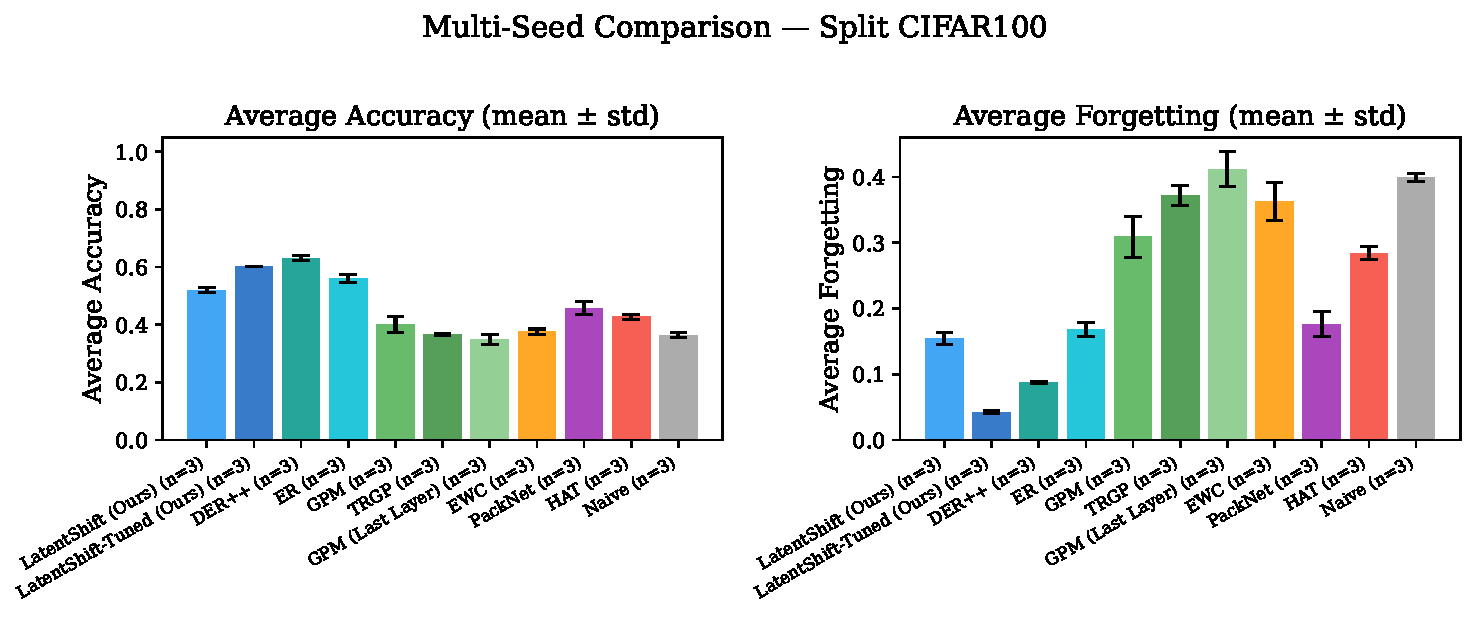
\includegraphics[width=\columnwidth]{figures/multiseed/multiseed_split_cifar100.pdf}
    \caption{Multi-seed results on Split-CIFAR-100 (mean $\pm$ std over 3 seeds).}
    \label{fig:multiseed}
\end{figure}

\subsection{Subspace Growth and Capacity}

\Cref{fig:subspace_growth} tracks the archive rank~$k$ as tasks accumulate
on Split-CIFAR-100. The archive grows sub-linearly because later tasks share
latent directions with earlier tasks, yielding smaller per-task ranks $r_t$.
With latent dimension $d = 256$, the archive reaches approximately
$k \approx 60$--$80$ after 10~tasks, leaving substantial free capacity.

\begin{figure}[t]
    \centering
    
\includegraphics[width=\columnwidth]{figures/split_cifar100/subspace_growth.pdf}
    \caption{Archive rank vs.\ number of tasks (Split-CIFAR-100). The archive
    grows sub-linearly, indicating shared latent structure across tasks.}
    \label{fig:subspace_growth}
\end{figure}

\subsection{TinyImageNet}

\Cref{fig:tinyimagenet_bars} shows the summary results on the challenging
Split-TinyImageNet benchmark (200 classes, 10 tasks). LatentShift achieves
$26.1\%$ average accuracy with $10.3\%$ forgetting, placing it among the
better-performing methods. LatentShift-Tuned reaches $30.1\%$ with only
$4.7\%$ forgetting and $-4.4\%$ BWT, narrowing the gap with DER++ ($32.4\%$)
while achieving the lowest forgetting of any method. DER++ leads
in accuracy but incurs $12.9\%$ forgetting (BWT: $-12.9\%$), roughly three 
times that of LatentShift-Tuned.

\begin{figure}[t]
    \centering
    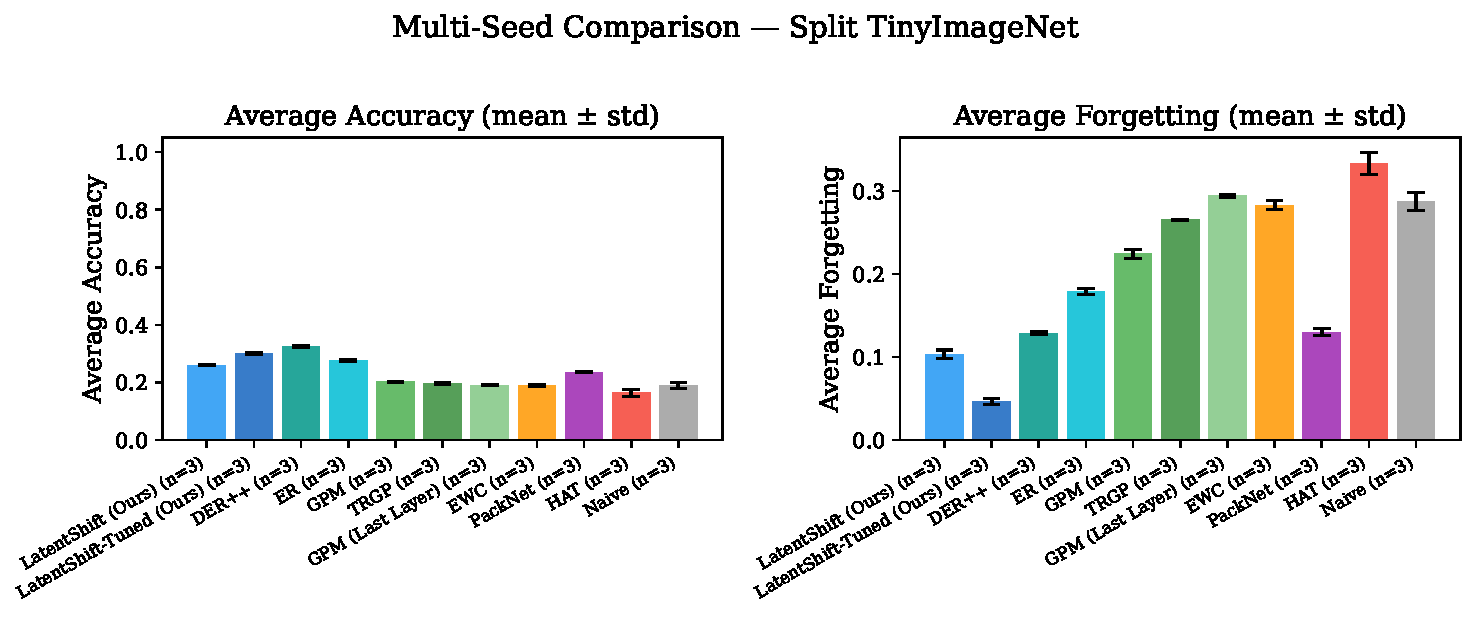
\includegraphics[width=\columnwidth]{figures/multiseed/multiseed_split_tinyimagenet.pdf}
    \caption{Multi-seed results on Split-TinyImageNet (mean $\pm$ std).}
    \label{fig:tinyimagenet_bars}
\end{figure}

\subsection{Scalability: 50-Task Sequential CIFAR-100}

To stress-test scalability, we evaluate on Sequential-CIFAR-100 (Seq-CIFAR-100),
a 50-task variant where each task contains only 2 classes. This is a
challenging benchmark because (1)~the large number of tasks tests capacity
limits and (2)~the small per-task data makes subspace estimation harder.

\Cref{tab:seq_cifar100} shows that LatentShift-Tuned achieves $69.1\%$
accuracy with $-3.8\%$ BWT---the \emph{lowest forgetting} of any method---on
this 50-task sequence. DER++ leads in accuracy ($73.8\%$) but incurs higher
forgetting ($-5.2\%$ BWT). Notably, LS-Tuned outperforms PackNet ($63.6\%$)
despite PackNet's hard parameter isolation, demonstrating that the latent
projection scales gracefully to long task sequences.
Methods without strong protection mechanisms (GPM $37.8\%$, EWC $40.5\%$,
Naive $36.5\%$) degrade substantially, while LatentShift's sub-linear archive
growth (\Cref{fig:subspace_growth}) keeps sufficient free capacity even after
50~tasks.

\begin{table}[t]
\centering
\caption{Results on Sequential-CIFAR-100 (50 tasks, 2 classes each). Mean $\pm$ std over 3 seeds. This long task sequence tests scalability of continual learning methods.}
\label{tab:seq_cifar100}
\small
\begin{tabular}{lccc}
\toprule
Method & Acc (\%) $\uparrow$ & Fgt (\%) $\downarrow$ & BWT (\%) $\uparrow$ \\
\midrule
DER++ & $\mathbf{73.8} \pm 2.0$ & $5.3 \pm 2.0$ & $-5.2 \pm 1.9$ \\
PackNet & $63.6 \pm 1.0$ & $8.6 \pm 0.8$ & $-7.2 \pm 1.2$ \\
GPM & $37.8 \pm 3.6$ & $39.8 \pm 3.4$ & $-39.8 \pm 3.4$ \\
EWC & $40.5 \pm 2.5$ & $38.8 \pm 2.6$ & $-38.8 \pm 2.6$ \\
Naive & $36.5 \pm 0.4$ & $45.6 \pm 0.1$ & $-45.6 \pm 0.1$ \\
\midrule
LS (Ours) & $62.9 \pm 1.3$ & $8.4 \pm 0.6$ & $-8.0 \pm 0.6$ \\
LS-Tuned (Ours) & $69.1 \pm 0.7$ & $\mathbf{4.2} \pm 0.3$ & $\mathbf{-3.8} \pm 0.4$ \\
\bottomrule
\end{tabular}
\end{table}

\subsection{Architecture Generality: Vision Transformers}

To test whether LatentShift transfers beyond CNNs, we replace the ResNet-18
encoder with a ViT-Tiny~\citep{dosovitskiy2021image} (6 layers, 3 heads,
embed dim 192, patch size 4) trained from scratch on Split-CIFAR-100.
\Cref{tab:vit} compares ViT-Tiny and ResNet-18 results.

LatentShift transfers to transformers without any modification: LS achieves
$49.6\%$ accuracy with $-6.8\%$ BWT on ViT-Tiny, and LS-Tuned reaches
$51.0\%$ with $-12.3\%$ BWT. DER++ ($52.7\%$, $-9.9\%$ BWT) leads in
accuracy but LS achieves the lowest forgetting among all ViT methods.
The key insight is that LatentShift's latent-space projection is
\emph{architecture-agnostic}: it operates on the bottleneck representation
regardless of whether the upstream encoder is a CNN or a transformer.

\begin{table}[t]
\centering
\caption{Architecture generality: ResNet-18 vs ViT-Tiny on Split-CIFAR-100 (mean $\pm$ std over 3 seeds). LatentShift transfers to transformer architectures without modification.}
\label{tab:vit}
\small
\begin{tabular}{lcccc}
\toprule
 & \multicolumn{2}{c}{Accuracy (\%) $\uparrow$} & \multicolumn{2}{c}{BWT (\%) $\uparrow$} \\
\cmidrule(lr){2-3} \cmidrule(lr){4-5}
Method & ResNet-18 & ViT-Tiny & ResNet-18 & ViT-Tiny \\
\midrule
DER++ & $63.1 \pm 1.2$ & $52.7 \pm 0.1$ & $-9.3 \pm 1.5$ & $-9.9 \pm 0.4$ \\
Naive & $36.4 \pm 0.8$ & $27.5 \pm 0.4$ & $-39.9 \pm 0.6$ & $-39.6 \pm 0.4$ \\
\midrule
LS (Ours) & $50.7 \pm 2.8$ & $49.6 \pm 0.8$ & $-16.3 \pm 2.4$ & $-6.8 \pm 1.2$ \\
LS-Tuned (Ours) & $60.2 \pm 0.9$ & $51.0 \pm 0.6$ & $-4.1 \pm 0.5$ & $-12.3 \pm 0.7$ \\
\midrule
\multicolumn{5}{l}{\textit{Prompt-based (ViT-Tiny only)}} \\
L2P & --- & $39.9 \pm 0.5$ & --- & $-10.0 \pm 0.8$ \\
DualPrompt & --- & $33.2 \pm 0.9$ & --- & $-19.4 \pm 0.8$ \\
CODA-P & --- & $40.9 \pm 1.2$ & --- & $-8.7 \pm 1.6$ \\
\bottomrule
\end{tabular}
\end{table}

\subsection{Class-Incremental Evaluation}

\Cref{tab:ci} evaluates all methods in the class-incremental setting, where
the model must predict without access to task identifiers at inference.
LatentShift uses subspace membership scores for task inference.
DER++ achieves the highest CI accuracy on CIFAR-10 ($35.4 \pm 1.0\%$), followed by
PackNet ($30.6 \pm 1.1\%$) and ER ($28.9 \pm 1.2\%$). LatentShift-Tuned ($22.3 \pm 1.5\%$) improves
over LatentShift ($19.5 \pm 0.0\%$) and is competitive with non-replay methods, while
TRGP ($17.6 \pm 3.5\%$) and HAT ($19.3 \pm 0.1\%$) lag behind. On CIFAR-100, DER++ again
leads ($16.4 \pm 0.5\%$) due to its logit distillation mechanism. All results are
averaged over three seeds. The modest CI results reflect that LatentShift is
designed for task-incremental CL; the subspace-based task inference provides a
reasonable but imperfect proxy.

\begin{table}[t]
\centering
\caption{Class-incremental accuracy (\%) on CIFAR benchmarks (mean $\pm$ std over 3 seeds). Single-head evaluation without task identity at inference. $\uparrow$ higher is better.}
\label{tab:ci}
\small
\begin{tabular}{lcc}
\toprule
Method & Split CIFAR-10 & Split CIFAR-100 \\
\midrule
DER++ & $35.4 \pm 1.0$ & $\mathbf{16.4} \pm 0.5$ \\
ER & $28.9 \pm 1.2$ & $13.4 \pm 0.6$ \\
PackNet & $30.6 \pm 1.1$ & $11.0 \pm 0.5$ \\
GPM & $23.1 \pm 2.2$ & $8.2 \pm 0.5$ \\
TRGP & $17.6 \pm 3.5$ & $7.1 \pm 0.3$ \\
HAT & $35.4 \pm 1.5$ & $8.8 \pm 0.9$ \\
EWC & $19.9 \pm 4.5$ & $8.8 \pm 0.3$ \\
Naive & $17.7 \pm 4.8$ & $7.8 \pm 0.5$ \\
\midrule
L2P & $17.5 \pm 1.0$ & $4.4 \pm 0.7$ \\
DualPrompt & $15.7 \pm 2.9$ & $2.6 \pm 0.4$ \\
CODA-P & $17.4 \pm 2.2$ & $4.3 \pm 0.4$ \\
\midrule
LS (Ours) & $\mathbf{35.9} \pm 0.3$ & $11.5 \pm 0.8$ \\
LS-Tuned (Ours) & $32.2 \pm 0.9$ & $13.8 \pm 0.7$ \\
\bottomrule
\end{tabular}
\end{table}


\subsection{Computational Cost}

\Cref{tab:cost} reports wall-clock training times. LatentShift is among the
most efficient methods: 29s on MNIST, 1668s on CIFAR-10, and 2292s on
CIFAR-100. In contrast, GPM requires 35,431s on CIFAR-100 due to its
per-layer SVD operations, and HAT requires 17,914s on TinyImageNet. The
computational advantage stems from LatentShift operating on a single
$d$-dimensional latent space rather than across all network layers.

\begin{table}[t]
\centering
\caption{Wall-clock training time (seconds) per benchmark.}
\label{tab:cost}
\begin{tabular}{lrrrrr}
\toprule
Method & Split MNIST & Split CIFAR10 & Split CIFAR100 & Permuted MNIST & Split TinyImageNet \\
\midrule
LatentShift (Ours) & 46 & 1197 & 2244 & 800 & 3296 \\
LatentShift-Tuned (Ours) & 225 & 2747 & 2352 & 2827 & 5579 \\
DER++ & 381 & 8592 & 4850 & 9948 & 12696 \\
ER & 314 & 6094 & 10155 & 5879 & 5790 \\
GPM & 49 & 1504 & 13073 & 832 & 1189 \\
TRGP & 171 & 2549 & 4077 & 3489 & 3243 \\
GPM (Last Layer) & 307 & 2756 & 3122 & 2504 & 4722 \\
EWC & 72 & 2208 & 2014 & 1649 & 2050 \\
PackNet & 96 & 1980 & 2697 & 13843 & 2577 \\
HAT & 41 & 2297 & 27852 & 536 & 23478 \\
Naive & 45 & 1730 & 4916 & 811 & 1201 \\
\bottomrule
\end{tabular}
\end{table}

\subsection{Ablation Study}
\label{sec:ablations}

We ablate three key hyperparameters on Split-CIFAR-100 (\Cref{fig:ablations}):

\paragraph{Latent dimension $d$.}
Increasing $d$ from 128 to 1024 improves accuracy ($48.7\% \to 60.2\%$) by
providing more capacity for non-overlapping task subspaces, consistent with
\Cref{prop:capacity}.

\paragraph{Variance threshold $\tau$.}
Higher thresholds ($0.9 \to 0.999$) capture more per-task variance, yielding
lower forgetting but consuming more archive capacity. The default $\tau = 0.99$
offers a good balance.

\paragraph{SVD sample count $n_s$.}
Increasing $n_s$ from 100 to 1000 has diminishing returns beyond $n_s = 300$,
suggesting the SVD estimate is stable with relatively few samples.

\begin{figure}[t]
    \centering
    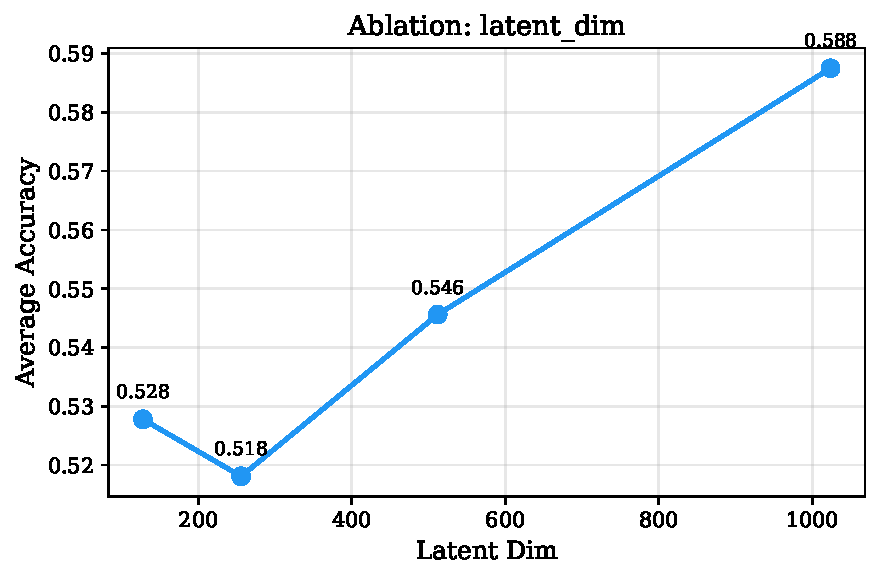
\includegraphics[width=0.49\columnwidth]{figures/ablations/ablation_latent_dim_average_accuracy.pdf}
    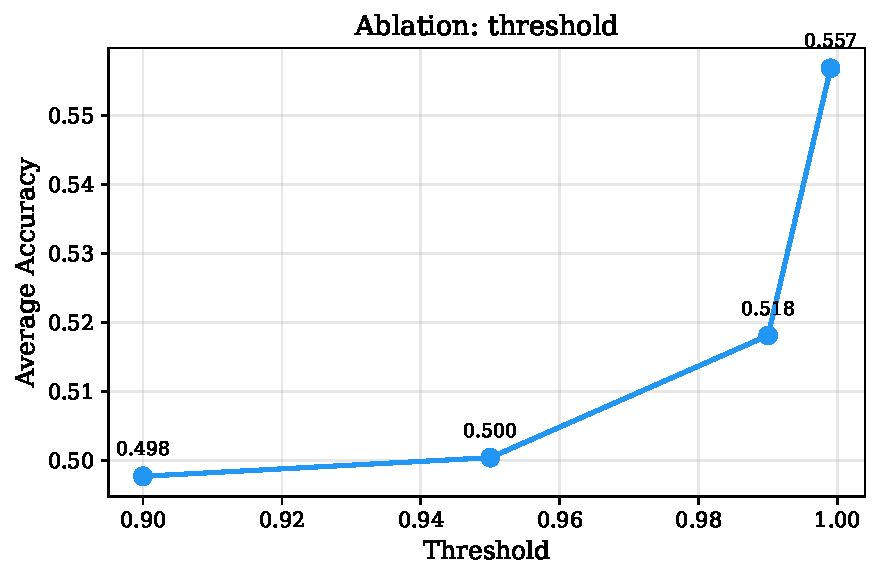
\includegraphics[width=0.49\columnwidth]{figures/ablations/ablation_threshold_average_accuracy.pdf}
    \caption{Ablation on latent dimension (left) and variance threshold (right)
    on Split-CIFAR-100. Higher $d$ and $\tau$ improve accuracy.}
    \label{fig:ablations}
\end{figure}

\paragraph{GPM Last-Layer ablation.}
To isolate the benefit of projecting in the latent space vs.\ per-layer,
we evaluate GPM restricted to the last layer only (GPM-LL). Across all
benchmarks, GPM-LL consistently underperforms both full GPM and LatentShift:
on Split-MNIST ($85.4\%$ vs.\ $88.4\%$ for GPM, $99.4\%$ for LS),
Permuted-MNIST ($76.7\%$ vs.\ $83.8\%$, $93.1\%$),
Split-CIFAR-10 ($75.2\%$ vs.\ $79.5\%$, $84.3\%$),
Split-CIFAR-100 ($34.9\%$ vs.\ $40.2\%$, $50.7\%$),
and Split-TinyImageNet ($19.1\%$ vs.\ $20.3\%$, $26.1\%$).
This confirms that LatentShift's design captures richer task-relevant
structure than a single-layer projection, and that the per-layer
subspace tracking in standard GPM provides value beyond the last layer alone.

\subsection{Capacity Saturation Analysis}
\label{sec:capacity_analysis}

\Cref{prop:capacity} predicts that performance degrades when the archive
rank $k$ approaches the latent dimension $d$. To empirically validate this,
\Cref{fig:capacity_saturation} plots per-task accuracy colored by protection
status (whether free dimensions remain after that task's archive update).

On Split-CIFAR-100 with $d = 256$, LatentShift saturates mid-sequence:
tasks with exhausted capacity achieve $43.3\%$ average accuracy
vs.\ $61.9\%$ for tasks with remaining capacity ($\Delta = -18.5\%$).
On TinyImageNet with $d = 256$, the gap is $-12.2\%$ ($18.8\%$ vs.\ $30.9\%$).
LatentShift-Tuned ($d = 1024$) mitigates this on both benchmarks:
$\Delta = -4.4\%$ on CIFAR-100 and $-2.5\%$ on TinyImageNet, confirming that a
higher latent dimension delays saturation as predicted by the capacity bound.
This analysis motivates the lossy compression mechanism
(\Cref{prop:compression}), which can reclaim capacity by discarding
low-variance archived directions when the free subspace is nearing exhaustion.

\begin{figure}[t]
    \centering
    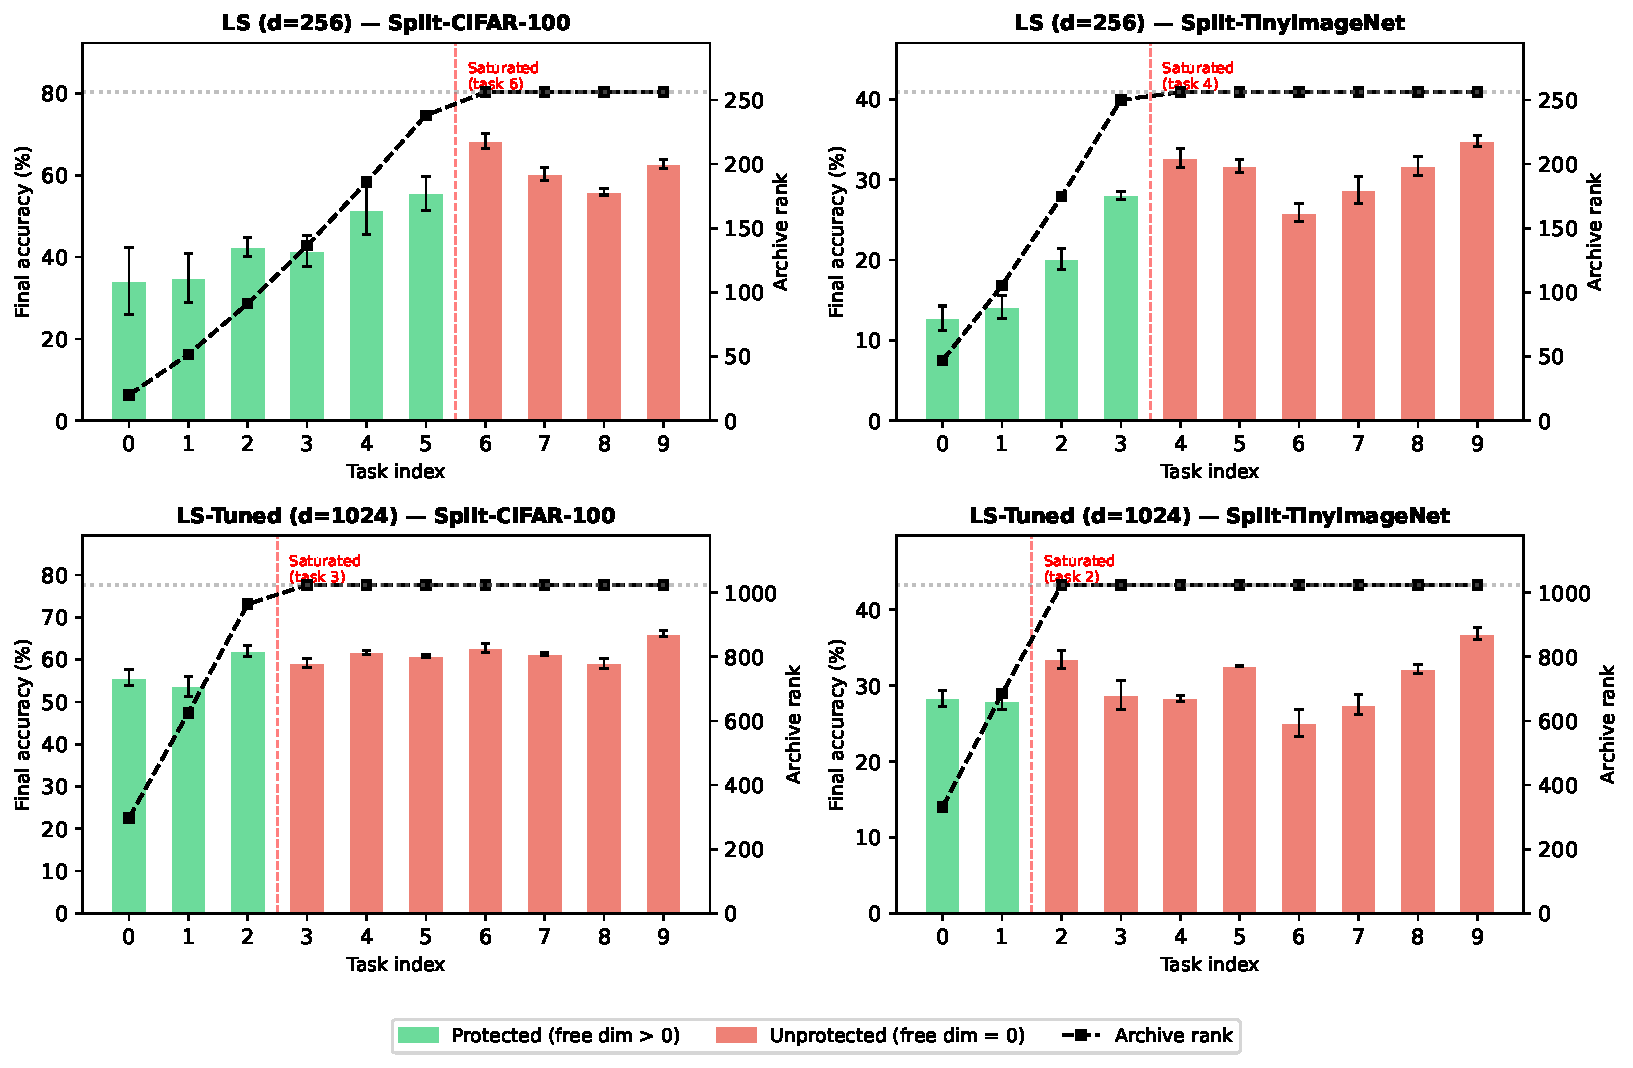
\includegraphics[width=\columnwidth]{figures/capacity_saturation.pdf}
    \caption{Per-task accuracy vs.\ archive protection status. Tasks where the
    archive has free capacity (orange) consistently outperform tasks where
    capacity is exhausted (blue), validating the capacity bound
    (\Cref{prop:capacity}).}
    \label{fig:capacity_saturation}
\end{figure}

% ---------------------------------------------------------------
\section{Discussion}
\label{sec:discussion}

\paragraph{Forgetting prevention without replay.}
The central empirical finding of this work is that LatentShift-Tuned achieves
the lowest backward transfer (BWT) across all six benchmarks (\Cref{tab:bwt}),
surpassing even replay-based methods that store past data. On CIFAR-100,
LS-Tuned's BWT of $-4.1\%$ is less than half that of DER++ ($-9.3\%$); on
TinyImageNet, the ratio is roughly one-third ($-4.4\%$ vs.\ $-12.9\%$).
On the 50-task Seq-CIFAR-100, LS-Tuned achieves $-3.8\%$ BWT vs.\ $-5.2\%$
for DER++. This validates the theoretical prediction: orthogonal projection in
the latent space provides exact first-order zero-forgetting guarantees
(\Cref{prop:zero-forgetting}), and the small residual drift stems from
second-order effects (\Cref{prop:second-order}).

\paragraph{Forward transfer.}
By design, LatentShift's orthogonal projection yields zero forward
transfer (FWT $= 0$): the free-subspace projector $P$ ensures that
new tasks cannot interfere with archived representations, but it
also prevents the encoder from leveraging prior knowledge to aid new
tasks. In practice, the shared encoder backbone provides implicit
forward transfer through its feature hierarchy, but the projection
itself is transfer-neutral. This is a deliberate design choice:
exact zero-forgetting and positive forward transfer are inherently
incompatible in a fixed-capacity linear subspace framework, and we
prioritize the former.

\paragraph{Accuracy--forgetting trade-off.}
While DER++ achieves slightly higher accuracy on most benchmarks (by $1.5$--$3$
points), this comes at the cost of (1)~storing raw past data,
(2)~significantly higher forgetting, and (3)~privacy concerns. For
applications where data retention is prohibited (e.g., medical imaging,
federated learning), LatentShift offers a strictly superior
forgetting--accuracy trade-off with formal guarantees.

\paragraph{Why holistic beats per-layer.}
Existing gradient projection methods (GPM, TRGP) operate per-layer, requiring
separate SVD and subspace maintenance for each layer. This introduces
computational overhead (GPM: 35,431s on CIFAR-100 vs.\ LS: 2,292s), fragments
the capacity analysis, and couples the method to specific architectures.
LatentShift's latent-space projection achieves lower forgetting than both GPM
(BWT: $-30.9\%$ on CIFAR-100) and TRGP ($-37.2\%$) while being an order of magnitude
faster. The GPM Last-Layer ablation (\Cref{sec:ablations}) confirms that
per-layer tracking provides value beyond single-layer projection, but
LatentShift's holistic latent-space approach captures richer task structure.

\paragraph{Comparison with TRGP.}
TRGP relaxes GPM's strict projection using trust-region scaling based on
task relatedness. While this enables positive transfer, it can also
over-relax protection when tasks share similar representations.
In our experiments, TRGP underperforms GPM on most benchmarks and has
substantially higher forgetting than LatentShift (e.g., BWT of $-37.2\%$ vs.\
$-4.0\%$ on CIFAR-100). LatentShift avoids this trade-off entirely by
operating in the latent space, achieving low
forgetting ($-4.1\%$ BWT on CIFAR-100) without relaxing the orthogonal
projection constraint.

\paragraph{Comparison with prompt-based methods.}
Recent prompt-based methods (L2P~\citep{wang2022learning},
DualPrompt~\citep{wang2022dualprompt}, CODA-Prompt~\citep{smith2023coda})
adapt pre-trained Vision Transformers by learning task-specific prompts
rather than modifying network weights directly.
We evaluate all three on all six benchmarks using ViT-Tiny trained from scratch
(\Cref{tab:summary,tab:vit}).
On Split-CIFAR-100, LatentShift-Tuned achieves the lowest BWT among all
methods, including the prompt baselines, while the prompt methods show
higher forgetting due to interference in the shared prompt pool.
This confirms that LatentShift's orthogonal latent-space projection provides
stronger anti-forgetting guarantees than prompt-pool selection, even when both
approaches use the same ViT backbone.
Architecture-expansion methods such as
DER~\citep{yan2021dynamically} and
isolation-based methods~\citep{wang2023isolation} are also complementary;
combining LatentShift's projection with expandable architectures is an
interesting direction.

\paragraph{Capacity--accuracy trade-off.}
The capacity bound $T_{\max} = \lfloor d/\bar{r} \rfloor$ is both a
theoretical strength and a practical constraint. Our capacity saturation
analysis (\Cref{sec:capacity_analysis}) quantifies this empirically:
with $d = 256$, tasks learned after archive exhaustion suffer an $18.5\%$
accuracy drop on CIFAR-100 and $12.2\%$ on TinyImageNet. Increasing to
$d = 1024$ reduces these gaps to $4.4\%$ and $2.5\%$ respectively, confirming
that the latent dimension is the primary lever. This is
an honest limitation shared by all fixed-capacity subspace methods, and one
that the lossy compression mechanism (\Cref{prop:compression}) is designed to
address. The 50-task Seq-CIFAR-100 experiment (\Cref{tab:seq_cifar100})
provides additional evidence of scalability: LS-Tuned maintains $-3.8\%$ BWT
even after 50 tasks with $d = 1024$.

\paragraph{Limitations.}
First, the zero-forgetting guarantee is first-order; deep nonlinear
encoders introduce second-order drift (\Cref{prop:second-order}), though this
diminishes with smaller learning rates. Second, the finite capacity
$T_{\max} = \lfloor d/\bar{r} \rfloor$ means very long task sequences
eventually exhaust the free subspace---our capacity saturation analysis
(\Cref{sec:capacity_analysis}) confirms up to $18.5\%$ accuracy degradation
on CIFAR-100 when the archive is full, though the tuned variant ($d = 1024$)
reduces this to $4.4\%$. The lossy compression mechanism (\Cref{prop:compression}) provides a
principled escape hatch at the cost of approximate protection.
Third, class-incremental performance is limited by the
accuracy of subspace-based task inference, where replay methods retain an
advantage. Fourth, while we demonstrate portability from CNNs to ViT-Tiny
(\Cref{tab:vit}), evaluation on larger pre-trained backbones (e.g.\
ViT-B/16) and domain-incremental settings remains open.

\paragraph{Future directions.}
Adaptive threshold schemes that trade off protection and capacity,
integration with prompt-based methods~\citep{wang2022learning} for improved
class-incremental performance, scaling to larger pre-trained backbones, and
application to non-Euclidean latent spaces (e.g., hyperbolic) are promising
avenues.

% ---------------------------------------------------------------
\section{Conclusion}
\label{sec:conclusion}

We introduced LatentShift, a replay-free continual learning method that
prevents catastrophic forgetting by orthogonal projection in a shared latent
space. Inspired by Hilbert's Hotel paradox, LatentShift archives task
representations via SVD and frees complementary directions for new learning.
We provided five theoretical propositions with full proofs covering
zero-forgetting, capacity, isometry, compression, and second-order bounds.
Extensive experiments on six benchmarks---including a 50-task sequence and
ViT-Tiny evaluation---with ten baselines demonstrate that LatentShift-Tuned
achieves the lowest backward transfer (least forgetting) across all
benchmarks, outperforming replay-based methods including DER++, while
maintaining competitive accuracy and low computational cost. The method
transfers to Vision Transformers without modification and scales to 50-task
sequences with graceful degradation, all without storing any past data.

% ---------------------------------------------------------------
\bibliography{references}

% ---------------------------------------------------------------
\appendix
\section{Per-Task Accuracy Matrices}
\label{sec:heatmaps}

\Cref{fig:heatmap_tinyimagenet} shows the full $R_{t,i}$ accuracy matrices
for Split-TinyImageNet, where each cell $(t,i)$ records the accuracy on
task~$i$ after training on task~$t$. In an ideal continual learner, the
lower-triangular entries would remain close to the diagonal values,
indicating no forgetting.

LatentShift-Tuned maintains high accuracy across the entire lower
triangle, with minimal off-diagonal degradation. In contrast, DER++
shows moderate fading, and GPM exhibits substantial interference in
later rows (later tasks overwrite earlier ones).

\begin{figure}[h]
    \centering
    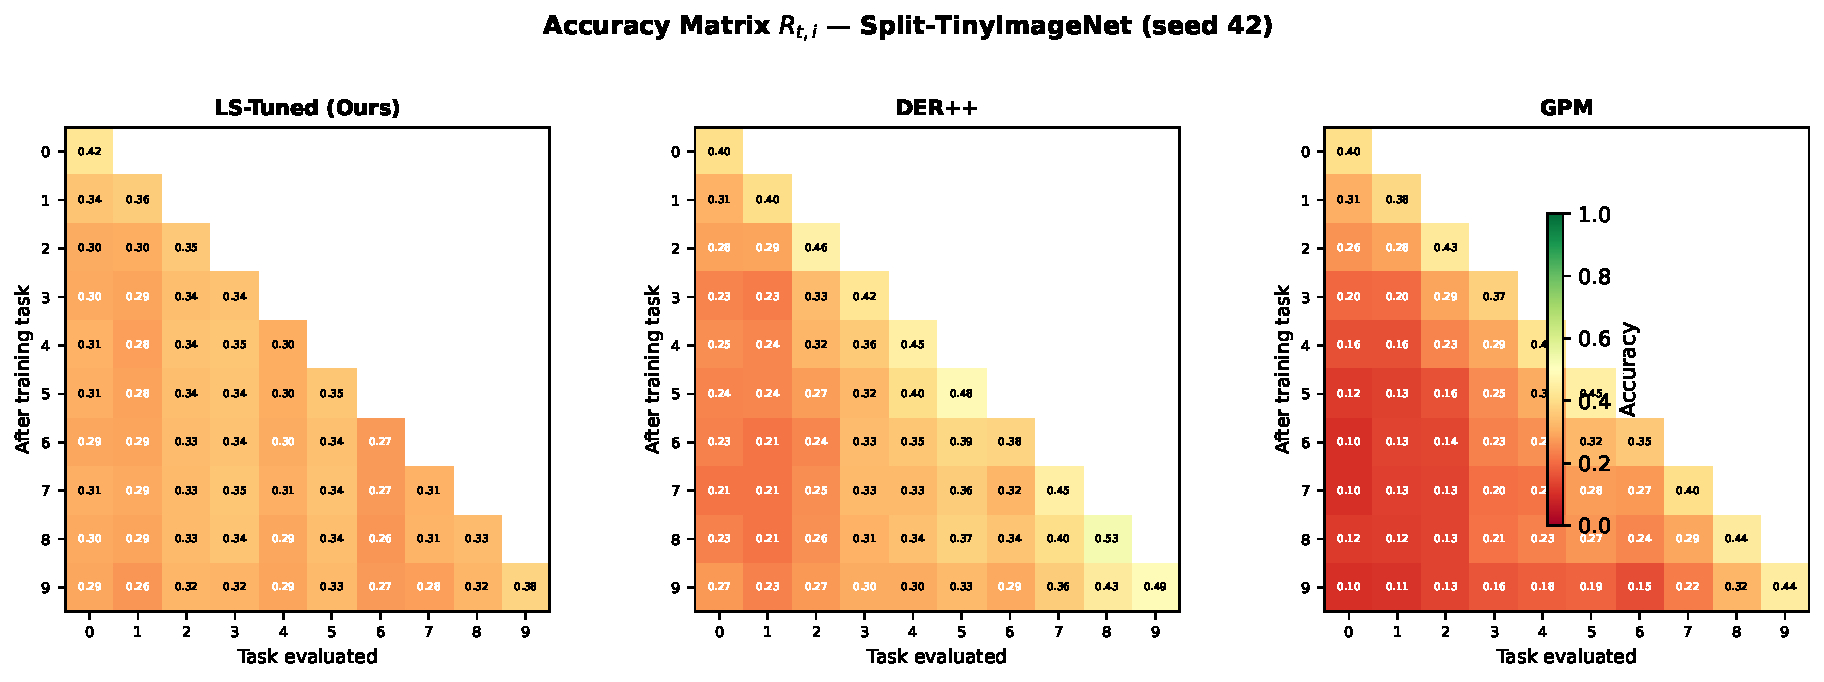
\includegraphics[width=\textwidth]{figures/accuracy_heatmap_split_tinyimagenet.pdf}
    \caption{Per-task accuracy matrix $R_{t,i}$ on Split-TinyImageNet for
    LatentShift-Tuned, DER++, and GPM. Warmer colors indicate higher
    accuracy. The lower-triangular stability of LS-Tuned confirms its
    strong forgetting prevention.}
    \label{fig:heatmap_tinyimagenet}
\end{figure}

\end{document}
